% DSA5208 Project 2 report. Build: cd report && tectonic DSA5208_Project2_Report.tex
% Every number comes from generated/values.tex or generated/tab_*.tex, written by src/report_macros.py from the
% pipeline's outputs; checks/requirements_check.py refuses a release with a hand-typed number.
\documentclass[10pt,a4paper]{article}
\linespread{1.06}
\usepackage[a4paper,margin=2.2cm]{geometry}
\usepackage{lmodern}
\usepackage[T1]{fontenc}
\PassOptionsToPackage{hyphens}{url}
\usepackage{microtype,booktabs,array,tabularx,xcolor,enumitem,caption,float,amsmath,amssymb,graphicx}
\usepackage[hidelinks]{hyperref}
\usepackage{titlesec}
\titleformat{\section}{\large\bfseries\sffamily}{\thesection}{0.6em}{}
\titleformat{\subsection}{\normalsize\bfseries\sffamily}{\thesubsection}{0.6em}{}
\titlespacing*{\section}{0pt}{1.4ex plus .4ex}{0.7ex}
\titlespacing*{\subsection}{0pt}{1.1ex plus .3ex}{0.5ex}
\setlist{itemsep=1pt,topsep=2pt,parsep=0pt}
\captionsetup{font=small,labelfont={bf,sf},skip=4pt}
\setlength{\parskip}{3pt}\setlength{\parindent}{0pt}
\renewcommand{\arraystretch}{1.1}
\graphicspath{{../figures/}}
\newcommand{\code}[1]{\texttt{#1}}  % write a CLI flag as -{}-flag: the empty group stops the -- ligature
\newcommand{\req}[1]{}
\newcommand{\setval}[2]{\expandafter\def\csname pv@#1\endcsname{#2}}
\newcommand{\val}[1]{\ifcsname pv@#1\endcsname\csname pv@#1\endcsname\else\errmessage{undefined generated value #1}\fi}
% generated by src/report_macros.py; do not edit
\setval{active_hours}{2}
\setval{ann.2017}{2{,}470}
\setval{ann.2018}{2{,}392}
\setval{ann.2019}{1{,}742}
\setval{ann.2020}{2{,}691}
\setval{ann.2021}{2{,}921}
\setval{ann.2022}{2{,}907}
\setval{ann.2023}{2{,}865}
\setval{ann.2024}{2{,}712}
\setval{ann_mean}{2{,}588}
\setval{bal_ratio_21_17}{1.18}
\setval{cand_th_hi1}{30}
\setval{cand_th_hi2}{40}
\setval{clean_in}{48{,}538{,}713}
\setval{clean_out}{48{,}538{,}627}
\setval{clean_removed}{86}
\setval{clim_pseudo}{20}
\setval{cloud.cluster}{dsa5208-p2}
\setval{cloud.cpu}{Intel(R) Xeon(R) CPU @ 2.80GHz}
\setval{cloud.disk}{80\,GB pd-balanced}
\setval{cloud.driver_mem}{8g}
\setval{cloud.dynalloc}{off}
\setval{cloud.exec_cores}{3}
\setval{cloud.exec_inst}{2}
\setval{cloud.exec_mem}{8g}
\setval{cloud.image}{3.0}
\setval{cloud.image_cfg}{3.0.3-debian13}
\setval{cloud.java}{21.0.12.1}
\setval{cloud.job_overhead}{29}
\setval{cloud.master}{yarn}
\setval{cloud.master_type}{n2-standard-4}
\setval{cloud.masters}{1}
\setval{cloud.n_runs}{9}
\setval{cloud.ncpu}{4}
\setval{cloud.os}{Debian GNU/Linux 13 (trixie)}
\setval{cloud.parallelism}{6}
\setval{cloud.python}{3.12.13}
\setval{cloud.ram}{16}
\setval{cloud.shuffle}{48}
\setval{cloud.spark}{4.1.2}
\setval{cloud.status}{run}
\setval{cloud.total_min}{44}
\setval{cloud.worker_type}{n2-standard-4}
\setval{cloud.workers}{2}
\setval{cloud.zone}{asia-southeast1-c}
\setval{cloud_ready}{yes}
\setval{coefB.isl_max_r30}{$+$0.44}
\setval{coefB.isl_wet30}{$+$0.28}
\setval{coefB.isl_wet_now}{$+$0.27}
\setval{coefB.log1p_r30}{$+$0.03}
\setval{coefB.log1p_r5}{$+$0.26}
\setval{coefB.log1p_theta}{$-$1.01}
\setval{coefB.mins_since_wet}{$-$0.45}
\setval{coefB.nb_max_r5}{$+$0.21}
\setval{coefB.nb_wet_now_frac}{$+$0.20}
\setval{coefB.top1}{log1p\_theta}
\setval{corr_freq}{0.95}
\setval{corr_int}{0.48}
\setval{corr_lon.imi}{$-$0.53}
\setval{corr_lon.imii}{$-$0.44}
\setval{corr_lon.ne}{$-$0.27}
\setval{corr_lon.sw}{$-$0.62}
\setval{corr_lon_all}{$-$0.51}
\setval{cov_days.2017}{365}
\setval{cov_days.2018}{326}
\setval{cov_days.2019}{354}
\setval{cov_days.2020}{364}
\setval{cov_days.2021}{362}
\setval{cov_days.2022}{365}
\setval{cov_days.2023}{357}
\setval{cov_days.2024}{366}
\setval{cov_share.2017}{81\,\%}
\setval{cov_share.2018}{78\,\%}
\setval{cov_share.2019}{89\,\%}
\setval{cov_share.2020}{75\,\%}
\setval{cov_share.2021}{88\,\%}
\setval{cov_share.2022}{94\,\%}
\setval{cov_share.2023}{87\,\%}
\setval{cov_share.2024}{87\,\%}
\setval{cov_share_max}{94\,\%}
\setval{cov_share_min}{75\,\%}
\setval{days.2018.aug}{3}
\setval{days.2018.feb}{21}
\setval{days.2019.jul}{27}
\setval{days.2021.jan}{28}
\setval{days.2023.jan}{23}
\setval{driest_month}{July}
\setval{driest_month_rate}{5.0}
\setval{dup_conflict}{0}
\setval{dup_n}{86}
\setval{env.cpu}{Apple M5}
\setval{env.driver_mem}{10g}
\setval{env.dynalloc}{at its default}
\setval{env.exec_cores}{--}
\setval{env.exec_inst}{--}
\setval{env.exec_mem}{--}
\setval{env.image}{--}
\setval{env.java}{17.0.20.1}
\setval{env.master}{local{[}10{]}}
\setval{env.n_runs}{12}
\setval{env.ncpu}{10}
\setval{env.os}{macOS 26.5.1}
\setval{env.parallelism}{10}
\setval{env.python}{3.11.17}
\setval{env.ram}{16}
\setval{env.shuffle}{64}
\setval{env.spark}{4.0.4}
\setval{env.status}{run}
\setval{env.total_min}{17}
\setval{example_th}{5}
\setval{f30_rows}{34{,}540{,}615}
\setval{f30pos.0}{2{,}074{,}113}
\setval{f30pos.0.5}{1{,}160{,}017}
\setval{f30pos.1}{804{,}510}
\setval{f30pos.10}{134{,}693}
\setval{f30pos.2}{537{,}008}
\setval{f30pos.20}{37{,}580}
\setval{f30pos.30}{10{,}282}
\setval{f30pos.40}{2{,}490}
\setval{f30pos.5}{281{,}076}
\setval{f30rate.0}{6.00\,\%}
\setval{f30rate.0.5}{3.36\,\%}
\setval{f30rate.1}{2.33\,\%}
\setval{f30rate.10}{0.39\,\%}
\setval{f30rate.2}{1.55\,\%}
\setval{f30rate.20}{0.11\,\%}
\setval{f30rate.30}{0.03\,\%}
\setval{f30rate.40}{0.01\,\%}
\setval{f30rate.5}{0.81\,\%}
\setval{first2017}{08:05}
\setval{first2017_day}{1 January}
\setval{first2017_raw}{08:04:59}
\setval{freq.2017}{2.83\,\%}
\setval{freq.2018}{2.88\,\%}
\setval{freq.2019}{1.94\,\%}
\setval{freq.2020}{3.04\,\%}
\setval{freq.2021}{3.04\,\%}
\setval{freq.2022}{3.09\,\%}
\setval{freq.2023}{3.20\,\%}
\setval{freq.2024}{3.05\,\%}
\setval{freqidx.2017}{98}
\setval{freqidx.2018}{100}
\setval{freqidx.2019}{67}
\setval{freqidx.2020}{105}
\setval{freqidx.2021}{106}
\setval{freqidx.2022}{107}
\setval{freqidx.2023}{111}
\setval{freqidx.2024}{106}
\setval{full_day_pct}{90}
\setval{gap_missed_pct}{10}
\setval{gap_ratio_pct}{15}
\setval{gauge_step}{0.2}
\setval{generated_at}{2026-10-17 20:32 +08}
\setval{grid}{0, 0.5, 1, 2, 5, 10, 20}
\setval{grid_max}{20}
\setval{grid_n}{7}
\setval{heavy_day_mm}{50}
\setval{heavy_hour_mm}{20}
\setval{heavy_hours_total}{13{,}116}
\setval{heavyd.2017}{21.7}
\setval{heavyd.2018}{24.0}
\setval{heavyd.2019}{15.3}
\setval{heavyd.2020}{25.6}
\setval{heavyd.2021}{35.1}
\setval{heavyd.2022}{30.0}
\setval{heavyd.2023}{31.7}
\setval{heavyd.2024}{30.2}
\setval{heavyh.2017}{28.4}
\setval{heavyh.2018}{34.3}
\setval{heavyh.2019}{19.9}
\setval{heavyh.2020}{33.5}
\setval{heavyh.2021}{38.2}
\setval{heavyh.2022}{39.0}
\setval{heavyh.2023}{35.3}
\setval{heavyh.2024}{32.2}
\setval{heavyh_mon.Apr}{42.7}
\setval{heavyh_mon.Aug}{29.5}
\setval{heavyh_mon.Dec}{36.4}
\setval{heavyh_mon.Feb}{23.1}
\setval{heavyh_mon.Jan}{26.3}
\setval{heavyh_mon.Jul}{22.7}
\setval{heavyh_mon.Jun}{34.8}
\setval{heavyh_mon.Mar}{31.8}
\setval{heavyh_mon.May}{35.5}
\setval{heavyh_mon.Nov}{51.9}
\setval{heavyh_mon.Oct}{30.5}
\setval{heavyh_mon.Sep}{32.6}
\setval{horizon}{30}
\setval{implausible_mm}{50}
\setval{index_base}{100}
\setval{ing_missing_years}{0}
\setval{ing_rows.2017}{5{,}256{,}106}
\setval{ing_rows.2018}{4{,}594{,}246}
\setval{ing_rows.2019}{5{,}026{,}862}
\setval{ing_rows.2020}{6{,}334{,}473}
\setval{ing_rows.2021}{7{,}044{,}646}
\setval{ing_rows.2022}{7{,}133{,}230}
\setval{ing_rows.2023}{6{,}742{,}890}
\setval{ing_rows.2024}{6{,}406{,}260}
\setval{ing_st_max}{80}
\setval{ing_st_min}{54}
\setval{ing_stations.2017}{62}
\setval{ing_stations.2018}{56}
\setval{ing_stations.2019}{54}
\setval{ing_stations.2020}{80}
\setval{ing_stations.2021}{76}
\setval{ing_stations.2022}{72}
\setval{ing_stations.2023}{74}
\setval{ing_stations.2024}{70}
\setval{ing_total}{48{,}538{,}713}
\setval{int.2017}{10.0}
\setval{int.2018}{10.4}
\setval{int.2019}{10.2}
\setval{int.2020}{10.3}
\setval{int.2021}{10.9}
\setval{int.2022}{10.8}
\setval{int.2023}{10.2}
\setval{int.2024}{10.1}
\setval{intense_mmh}{30}
\setval{intense_share_all}{47\,\%}
\setval{intidx.2017}{96}
\setval{intidx.2018}{101}
\setval{intidx.2019}{98}
\setval{intidx.2020}{100}
\setval{intidx.2021}{105}
\setval{intidx.2022}{104}
\setval{intidx.2023}{98}
\setval{intidx.2024}{98}
\setval{intmon.Apr}{12.3}
\setval{intmon.Aug}{10.7}
\setval{intmon.Dec}{9.9}
\setval{intmon.Feb}{10.4}
\setval{intmon.Jan}{7.5}
\setval{intmon.Jul}{10.7}
\setval{intmon.Jun}{10.5}
\setval{intmon.Mar}{11.4}
\setval{intmon.May}{11.7}
\setval{intmon.Nov}{10.8}
\setval{intmon.Oct}{10.3}
\setval{intmon.Sep}{10.7}
\setval{intshare.Apr}{53\,\%}
\setval{intshare.Aug}{48\,\%}
\setval{intshare.Dec}{46\,\%}
\setval{intshare.Feb}{45\,\%}
\setval{intshare.Jan}{34\,\%}
\setval{intshare.Jul}{49\,\%}
\setval{intshare.Jun}{46\,\%}
\setval{intshare.Mar}{50\,\%}
\setval{intshare.May}{51\,\%}
\setval{intshare.Nov}{51\,\%}
\setval{intshare.Oct}{47\,\%}
\setval{intshare.Sep}{46\,\%}
\setval{jan21_first}{20:30}
\setval{jan21_first_day}{5 January}
\setval{jan21_gap_days}{1--4 January}
\setval{jan21_last}{07:55}
\setval{jan21_last_day}{1 January}
\setval{jan21_off_anom}{$+$70}
\setval{k_nb}{6}
\setval{low_cov_days}{15}
\setval{manom.2017.Apr}{$-$2}
\setval{manom.2017.Aug}{$-$27}
\setval{manom.2017.Dec}{$+$2}
\setval{manom.2017.Feb}{$+$3}
\setval{manom.2017.Jan}{$+$1}
\setval{manom.2017.Jul}{$-$16}
\setval{manom.2017.Jun}{$-$41}
\setval{manom.2017.Mar}{$-$14}
\setval{manom.2017.May}{$+$12}
\setval{manom.2017.Nov}{$+$4}
\setval{manom.2017.Oct}{$-$7}
\setval{manom.2017.Sep}{$-$8}
\setval{manom.2018.Apr}{$-$9}
\setval{manom.2018.Aug}{$-$93}
\setval{manom.2018.Dec}{$-$11}
\setval{manom.2018.Feb}{$-$47}
\setval{manom.2018.Jan}{$+$39}
\setval{manom.2018.Jul}{$-$28}
\setval{manom.2018.Jun}{$+$11}
\setval{manom.2018.Mar}{$-$32}
\setval{manom.2018.May}{$+$10}
\setval{manom.2018.Nov}{$+$1}
\setval{manom.2018.Oct}{$+$22}
\setval{manom.2018.Sep}{$-$23}
\setval{manom.2019.Apr}{$-$6}
\setval{manom.2019.Aug}{$-$81}
\setval{manom.2019.Dec}{$+$10}
\setval{manom.2019.Feb}{$-$66}
\setval{manom.2019.Jan}{$-$60}
\setval{manom.2019.Jul}{$-$60}
\setval{manom.2019.Jun}{$-$7}
\setval{manom.2019.Mar}{$-$44}
\setval{manom.2019.May}{$-$17}
\setval{manom.2019.Nov}{$-$35}
\setval{manom.2019.Oct}{$-$27}
\setval{manom.2019.Sep}{$-$57}
\setval{manom.2020.Apr}{$+$5}
\setval{manom.2020.Aug}{$+$13}
\setval{manom.2020.Dec}{$+$2}
\setval{manom.2020.Feb}{$-$36}
\setval{manom.2020.Jan}{$-$38}
\setval{manom.2020.Jul}{$+$42}
\setval{manom.2020.Jun}{$+$43}
\setval{manom.2020.Mar}{$-$39}
\setval{manom.2020.May}{$+$13}
\setval{manom.2020.Nov}{$-$5}
\setval{manom.2020.Oct}{$-$20}
\setval{manom.2020.Sep}{$+$40}
\setval{manom.2021.Apr}{$+$44}
\setval{manom.2021.Aug}{$+$115}
\setval{manom.2021.Dec}{$-$26}
\setval{manom.2021.Feb}{$-$78}
\setval{manom.2021.Jan}{$+$18}
\setval{manom.2021.Jul}{$+$37}
\setval{manom.2021.Jun}{$-$14}
\setval{manom.2021.Mar}{$+$30}
\setval{manom.2021.May}{$+$13}
\setval{manom.2021.Nov}{$-$13}
\setval{manom.2021.Oct}{$-$23}
\setval{manom.2021.Sep}{$+$22}
\setval{manom.2022.Apr}{$-$5}
\setval{manom.2022.Aug}{$+$22}
\setval{manom.2022.Dec}{$-$5}
\setval{manom.2022.Feb}{$+$44}
\setval{manom.2022.Jan}{$-$42}
\setval{manom.2022.Jul}{$-$24}
\setval{manom.2022.Jun}{$-$9}
\setval{manom.2022.Mar}{$+$31}
\setval{manom.2022.May}{$-$5}
\setval{manom.2022.Nov}{$+$12}
\setval{manom.2022.Oct}{$+$99}
\setval{manom.2022.Sep}{$+$10}
\setval{manom.2023.Apr}{$-$19}
\setval{manom.2023.Aug}{$-$36}
\setval{manom.2023.Dec}{$+$46}
\setval{manom.2023.Feb}{$+$136}
\setval{manom.2023.Jan}{$+$17}
\setval{manom.2023.Jul}{$+$65}
\setval{manom.2023.Jun}{$-$3}
\setval{manom.2023.Mar}{$+$45}
\setval{manom.2023.May}{$-$41}
\setval{manom.2023.Nov}{$-$5}
\setval{manom.2023.Oct}{$-$43}
\setval{manom.2023.Sep}{$-$16}
\setval{manom.2024.Apr}{$-$15}
\setval{manom.2024.Aug}{$-$33}
\setval{manom.2024.Dec}{$-$18}
\setval{manom.2024.Feb}{$-$12}
\setval{manom.2024.Jan}{$+$61}
\setval{manom.2024.Jul}{$-$48}
\setval{manom.2024.Jun}{$+$16}
\setval{manom.2024.Mar}{$-$17}
\setval{manom.2024.May}{$+$23}
\setval{manom.2024.Nov}{$+$32}
\setval{manom.2024.Oct}{$-$9}
\setval{manom.2024.Sep}{$+$5}
\setval{max5.2017}{18.0}
\setval{max5.2018}{15.6}
\setval{max5.2019}{15.4}
\setval{max5.2020}{20.6}
\setval{max5.2021}{26.4}
\setval{max5.2022}{37.2}
\setval{max5.2023}{17.6}
\setval{max5.2024}{15.9}
\setval{maxhour.2017}{91.2}
\setval{maxhour.2018}{86.4}
\setval{maxhour.2019}{88.0}
\setval{maxhour.2020}{106.0}
\setval{maxhour.2021}{90.5}
\setval{maxhour.2022}{140.2}
\setval{maxhour.2023}{98.5}
\setval{maxhour.2024}{90.0}
\setval{medmaxhour.2017}{53.6}
\setval{medmaxhour.2018}{55.2}
\setval{medmaxhour.2019}{53.8}
\setval{medmaxhour.2020}{58.1}
\setval{medmaxhour.2021}{62.4}
\setval{medmaxhour.2022}{63.6}
\setval{medmaxhour.2023}{58.4}
\setval{medmaxhour.2024}{59.2}
\setval{min_pos.2020}{0.197}
\setval{min_rate.imi}{0.09}
\setval{min_rate.imii}{0.09}
\setval{min_rate.ne}{0.10}
\setval{min_rate.sw}{0.07}
\setval{mono.Bgbt}{1.6\,\%}
\setval{mono.Bgbt.max}{0.67}
\setval{mr.2017.Apr}{8.2}
\setval{mr.2017.Aug}{4.5}
\setval{mr.2017.Dec}{8.6}
\setval{mr.2017.Feb}{5.4}
\setval{mr.2017.Jan}{8.0}
\setval{mr.2017.Jul}{4.2}
\setval{mr.2017.Jun}{4.6}
\setval{mr.2017.Mar}{5.9}
\setval{mr.2017.May}{7.8}
\setval{mr.2017.Nov}{10.9}
\setval{mr.2017.Oct}{6.4}
\setval{mr.2017.Sep}{6.6}
\setval{mr.2018.Apr}{7.6}
\setval{mr.2018.Aug}{0.5}
\setval{mr.2018.Dec}{7.5}
\setval{mr.2018.Feb}{2.8}
\setval{mr.2018.Jan}{10.9}
\setval{mr.2018.Jul}{3.6}
\setval{mr.2018.Jun}{8.7}
\setval{mr.2018.Mar}{4.7}
\setval{mr.2018.May}{7.6}
\setval{mr.2018.Nov}{10.7}
\setval{mr.2018.Oct}{8.3}
\setval{mr.2018.Sep}{5.5}
\setval{mr.2019.Apr}{7.8}
\setval{mr.2019.Aug}{1.2}
\setval{mr.2019.Dec}{9.3}
\setval{mr.2019.Feb}{1.8}
\setval{mr.2019.Jan}{3.1}
\setval{mr.2019.Jul}{2.0}
\setval{mr.2019.Jun}{7.3}
\setval{mr.2019.Mar}{3.9}
\setval{mr.2019.May}{5.8}
\setval{mr.2019.Nov}{6.9}
\setval{mr.2019.Oct}{5.0}
\setval{mr.2019.Sep}{3.1}
\setval{mr.2020.Apr}{8.7}
\setval{mr.2020.Aug}{7.0}
\setval{mr.2020.Dec}{8.6}
\setval{mr.2020.Feb}{3.4}
\setval{mr.2020.Jan}{4.9}
\setval{mr.2020.Jul}{7.1}
\setval{mr.2020.Jun}{11.2}
\setval{mr.2020.Mar}{4.2}
\setval{mr.2020.May}{7.8}
\setval{mr.2020.Nov}{10.0}
\setval{mr.2020.Oct}{5.4}
\setval{mr.2020.Sep}{10.0}
\setval{mr.2021.Apr}{12.0}
\setval{mr.2021.Aug}{13.2}
\setval{mr.2021.Dec}{6.3}
\setval{mr.2021.Feb}{1.2}
\setval{mr.2021.Jan}{9.3}
\setval{mr.2021.Jul}{6.8}
\setval{mr.2021.Jun}{6.8}
\setval{mr.2021.Mar}{9.0}
\setval{mr.2021.May}{7.9}
\setval{mr.2021.Nov}{9.2}
\setval{mr.2021.Oct}{5.2}
\setval{mr.2021.Sep}{8.7}
\setval{mr.2022.Apr}{8.0}
\setval{mr.2022.Aug}{7.5}
\setval{mr.2022.Dec}{8.1}
\setval{mr.2022.Feb}{7.6}
\setval{mr.2022.Jan}{4.6}
\setval{mr.2022.Jul}{3.8}
\setval{mr.2022.Jun}{7.2}
\setval{mr.2022.Mar}{9.1}
\setval{mr.2022.May}{6.6}
\setval{mr.2022.Nov}{11.8}
\setval{mr.2022.Oct}{13.5}
\setval{mr.2022.Sep}{7.8}
\setval{mr.2023.Apr}{6.7}
\setval{mr.2023.Aug}{3.9}
\setval{mr.2023.Dec}{12.4}
\setval{mr.2023.Feb}{12.4}
\setval{mr.2023.Jan}{9.2}
\setval{mr.2023.Jul}{8.2}
\setval{mr.2023.Jun}{7.6}
\setval{mr.2023.Mar}{10.1}
\setval{mr.2023.May}{4.1}
\setval{mr.2023.Nov}{10.0}
\setval{mr.2023.Oct}{3.9}
\setval{mr.2023.Sep}{6.0}
\setval{mr.2024.Apr}{7.0}
\setval{mr.2024.Aug}{4.1}
\setval{mr.2024.Dec}{6.9}
\setval{mr.2024.Feb}{4.6}
\setval{mr.2024.Jan}{12.7}
\setval{mr.2024.Jul}{2.6}
\setval{mr.2024.Jun}{9.2}
\setval{mr.2024.Mar}{5.7}
\setval{mr.2024.May}{8.6}
\setval{mr.2024.Nov}{13.9}
\setval{mr.2024.Oct}{6.2}
\setval{mr.2024.Sep}{7.5}
\setval{mrate.Apr}{8.3}
\setval{mrate.Aug}{6.2}
\setval{mrate.Dec}{8.5}
\setval{mrate.Feb}{5.3}
\setval{mrate.Jan}{7.9}
\setval{mrate.Jul}{5.0}
\setval{mrate.Jun}{7.9}
\setval{mrate.Mar}{6.9}
\setval{mrate.May}{7.0}
\setval{mrate.Nov}{10.5}
\setval{mrate.Oct}{6.8}
\setval{mrate.Sep}{7.1}
\setval{mss_active_sm}{4{,}272}
\setval{mss_bad_months}{4}
\setval{mss_big20}{101}
\setval{mss_big5}{319}
\setval{mss_cls.complete}{66.1\,\%}
\setval{mss_cls.network_outage}{1.7\,\%}
\setval{mss_cls.partial}{23.5\,\%}
\setval{mss_cls.station_absent_month}{7.7\,\%}
\setval{mss_cls.station_gap}{1.0\,\%}
\setval{mss_clsdays.complete}{88{,}443}
\setval{mss_clsdays.network_outage}{3{,}262}
\setval{mss_clsdays.partial}{32{,}561}
\setval{mss_clsdays.station_absent_month}{10{,}109}
\setval{mss_clsdays.station_gap}{1{,}467}
\setval{mss_corr}{0.991}
\setval{mss_days}{88{,}443}
\setval{mss_false_heavy}{2}
\setval{mss_gap_outage}{1.8\,\%}
\setval{mss_gap_partial}{25.5\,\%}
\setval{mss_gap_station}{1.0\,\%}
\setval{mss_heavy_off}{2{,}305}
\setval{mss_heavy_ours}{2{,}271}
\setval{mss_heavyrate_off.2017}{21.2}
\setval{mss_heavyrate_off.2018}{22.8}
\setval{mss_heavyrate_off.2019}{16.3}
\setval{mss_heavyrate_off.2020}{24.3}
\setval{mss_heavyrate_off.2021}{35.1}
\setval{mss_heavyrate_off.2022}{29.3}
\setval{mss_heavyrate_off.2023}{26.9}
\setval{mss_heavyrate_off.2024}{30.8}
\setval{mss_heavyrate_ours.2017}{20.9}
\setval{mss_heavyrate_ours.2018}{22.6}
\setval{mss_heavyrate_ours.2019}{15.7}
\setval{mss_heavyrate_ours.2020}{24.0}
\setval{mss_heavyrate_ours.2021}{34.4}
\setval{mss_heavyrate_ours.2022}{29.1}
\setval{mss_heavyrate_ours.2023}{26.5}
\setval{mss_heavyrate_ours.2024}{30.4}
\setval{mss_lg0.date}{2021-04-01}
\setval{mss_lg0.off}{0.0}
\setval{mss_lg0.ours}{318.2}
\setval{mss_lg0.st}{S36}
\setval{mss_lg1.date}{2021-01-20}
\setval{mss_lg1.off}{0.0}
\setval{mss_lg1.ours}{137.8}
\setval{mss_lg1.st}{S36}
\setval{mss_lg2.date}{2023-12-25}
\setval{mss_lg2.off}{134.0}
\setval{mss_lg2.ours}{0.6}
\setval{mss_lg2.st}{S104}
\setval{mss_mae}{0.086}
\setval{mss_maxdiff}{318.2}
\setval{mss_meandiff}{$-$0.061}
\setval{mss_missed_heavy}{13}
\setval{mss_month_median_ratio}{1.00}
\setval{mss_n_files}{4729}
\setval{mss_n_probe}{54}
\setval{mss_odd_list}{Feb 2018 (1.44), Aug 2020 (1.28)}
\setval{mss_odd_n}{2}
\setval{mss_outage_days}{64}
\setval{mss_ratio}{0.991}
\setval{mss_ratio_range_hi}{1.05}
\setval{mss_ratio_range_lo}{0.97}
\setval{mss_small}{5}
\setval{mss_spur.date}{2021-04-01}
\setval{mss_spur.off}{0.0}
\setval{mss_spur.ours}{318.2}
\setval{mss_spur.st}{S36}
\setval{mss_stations}{54}
\setval{mss_wet_disagree}{300}
\setval{mss_within02}{99.1\,\%}
\setval{mss_within1}{99.4\,\%}
\setval{mss_zero.date}{2023-12-25}
\setval{mss_zero.off}{134.0}
\setval{mss_zero.ours}{0.6}
\setval{mss_zero.st}{S104}
\setval{mssmissed.2017.Apr}{4\,\%}
\setval{mssmissed.2017.Aug}{5\,\%}
\setval{mssmissed.2017.Dec}{0\,\%}
\setval{mssmissed.2017.Feb}{0\,\%}
\setval{mssmissed.2017.Jan}{0\,\%}
\setval{mssmissed.2017.Jul}{0\,\%}
\setval{mssmissed.2017.Jun}{0\,\%}
\setval{mssmissed.2017.Mar}{1\,\%}
\setval{mssmissed.2017.May}{0\,\%}
\setval{mssmissed.2017.Nov}{2\,\%}
\setval{mssmissed.2017.Oct}{0\,\%}
\setval{mssmissed.2017.Sep}{0\,\%}
\setval{mssmissed.2018.Apr}{20\,\%}
\setval{mssmissed.2018.Aug}{99\,\%}
\setval{mssmissed.2018.Dec}{3\,\%}
\setval{mssmissed.2018.Feb}{3\,\%}
\setval{mssmissed.2018.Jan}{0\,\%}
\setval{mssmissed.2018.Jul}{0\,\%}
\setval{mssmissed.2018.Jun}{0\,\%}
\setval{mssmissed.2018.Mar}{0\,\%}
\setval{mssmissed.2018.May}{0\,\%}
\setval{mssmissed.2018.Nov}{3\,\%}
\setval{mssmissed.2018.Oct}{1\,\%}
\setval{mssmissed.2018.Sep}{1\,\%}
\setval{mssmissed.2019.Apr}{1\,\%}
\setval{mssmissed.2019.Aug}{0\,\%}
\setval{mssmissed.2019.Dec}{0\,\%}
\setval{mssmissed.2019.Feb}{2\,\%}
\setval{mssmissed.2019.Jan}{3\,\%}
\setval{mssmissed.2019.Jul}{30\,\%}
\setval{mssmissed.2019.Jun}{3\,\%}
\setval{mssmissed.2019.Mar}{0\,\%}
\setval{mssmissed.2019.May}{1\,\%}
\setval{mssmissed.2019.Nov}{12\,\%}
\setval{mssmissed.2019.Oct}{0\,\%}
\setval{mssmissed.2019.Sep}{0\,\%}
\setval{mssmissed.2020.Apr}{1\,\%}
\setval{mssmissed.2020.Aug}{1\,\%}
\setval{mssmissed.2020.Dec}{2\,\%}
\setval{mssmissed.2020.Feb}{0\,\%}
\setval{mssmissed.2020.Jan}{0\,\%}
\setval{mssmissed.2020.Jul}{0\,\%}
\setval{mssmissed.2020.Jun}{4\,\%}
\setval{mssmissed.2020.Mar}{0\,\%}
\setval{mssmissed.2020.May}{1\,\%}
\setval{mssmissed.2020.Nov}{1\,\%}
\setval{mssmissed.2020.Oct}{0\,\%}
\setval{mssmissed.2020.Sep}{0\,\%}
\setval{mssmissed.2021.Apr}{0\,\%}
\setval{mssmissed.2021.Aug}{1\,\%}
\setval{mssmissed.2021.Dec}{0\,\%}
\setval{mssmissed.2021.Feb}{0\,\%}
\setval{mssmissed.2021.Jan}{32\,\%}
\setval{mssmissed.2021.Jul}{3\,\%}
\setval{mssmissed.2021.Jun}{0\,\%}
\setval{mssmissed.2021.Mar}{1\,\%}
\setval{mssmissed.2021.May}{0\,\%}
\setval{mssmissed.2021.Nov}{0\,\%}
\setval{mssmissed.2021.Oct}{0\,\%}
\setval{mssmissed.2021.Sep}{0\,\%}
\setval{mssmissed.2022.Apr}{0\,\%}
\setval{mssmissed.2022.Aug}{11\,\%}
\setval{mssmissed.2022.Dec}{0\,\%}
\setval{mssmissed.2022.Feb}{1\,\%}
\setval{mssmissed.2022.Jan}{0\,\%}
\setval{mssmissed.2022.Jul}{0\,\%}
\setval{mssmissed.2022.Jun}{1\,\%}
\setval{mssmissed.2022.Mar}{0\,\%}
\setval{mssmissed.2022.May}{0\,\%}
\setval{mssmissed.2022.Nov}{1\,\%}
\setval{mssmissed.2022.Oct}{0\,\%}
\setval{mssmissed.2022.Sep}{0\,\%}
\setval{mssmissed.2023.Apr}{3\,\%}
\setval{mssmissed.2023.Aug}{4\,\%}
\setval{mssmissed.2023.Dec}{0\,\%}
\setval{mssmissed.2023.Feb}{1\,\%}
\setval{mssmissed.2023.Jan}{18\,\%}
\setval{mssmissed.2023.Jul}{1\,\%}
\setval{mssmissed.2023.Jun}{0\,\%}
\setval{mssmissed.2023.Mar}{1\,\%}
\setval{mssmissed.2023.May}{2\,\%}
\setval{mssmissed.2023.Nov}{0\,\%}
\setval{mssmissed.2023.Oct}{0\,\%}
\setval{mssmissed.2023.Sep}{1\,\%}
\setval{mssmissed.2024.Apr}{0\,\%}
\setval{mssmissed.2024.Aug}{8\,\%}
\setval{mssmissed.2024.Dec}{0\,\%}
\setval{mssmissed.2024.Feb}{0\,\%}
\setval{mssmissed.2024.Jan}{0\,\%}
\setval{mssmissed.2024.Jul}{0\,\%}
\setval{mssmissed.2024.Jun}{1\,\%}
\setval{mssmissed.2024.Mar}{1\,\%}
\setval{mssmissed.2024.May}{0\,\%}
\setval{mssmissed.2024.Nov}{3\,\%}
\setval{mssmissed.2024.Oct}{1\,\%}
\setval{mssmissed.2024.Sep}{0\,\%}
\setval{mssoff.2017.Apr}{8.96}
\setval{mssoff.2017.Aug}{4.64}
\setval{mssoff.2017.Dec}{9.04}
\setval{mssoff.2017.Feb}{5.69}
\setval{mssoff.2017.Jan}{8.31}
\setval{mssoff.2017.Jul}{4.16}
\setval{mssoff.2017.Jun}{4.30}
\setval{mssoff.2017.Mar}{6.26}
\setval{mssoff.2017.May}{7.99}
\setval{mssoff.2017.Nov}{10.78}
\setval{mssoff.2017.Oct}{6.36}
\setval{mssoff.2017.Sep}{6.51}
\setval{mssoff.2018.Apr}{7.30}
\setval{mssoff.2018.Aug}{2.92}
\setval{mssoff.2018.Dec}{7.54}
\setval{mssoff.2018.Feb}{1.92}
\setval{mssoff.2018.Jan}{11.09}
\setval{mssoff.2018.Jul}{3.61}
\setval{mssoff.2018.Jun}{8.77}
\setval{mssoff.2018.Mar}{4.64}
\setval{mssoff.2018.May}{7.62}
\setval{mssoff.2018.Nov}{10.84}
\setval{mssoff.2018.Oct}{8.29}
\setval{mssoff.2018.Sep}{6.09}
\setval{mssoff.2019.Apr}{7.39}
\setval{mssoff.2019.Aug}{1.10}
\setval{mssoff.2019.Dec}{9.28}
\setval{mssoff.2019.Feb}{1.81}
\setval{mssoff.2019.Jan}{3.14}
\setval{mssoff.2019.Jul}{2.38}
\setval{mssoff.2019.Jun}{7.52}
\setval{mssoff.2019.Mar}{3.85}
\setval{mssoff.2019.May}{5.92}
\setval{mssoff.2019.Nov}{6.44}
\setval{mssoff.2019.Oct}{5.10}
\setval{mssoff.2019.Sep}{3.16}
\setval{mssoff.2020.Apr}{8.79}
\setval{mssoff.2020.Aug}{5.53}
\setval{mssoff.2020.Dec}{8.71}
\setval{mssoff.2020.Feb}{3.33}
\setval{mssoff.2020.Jan}{4.77}
\setval{mssoff.2020.Jul}{6.66}
\setval{mssoff.2020.Jun}{10.11}
\setval{mssoff.2020.Mar}{4.30}
\setval{mssoff.2020.May}{7.90}
\setval{mssoff.2020.Nov}{9.68}
\setval{mssoff.2020.Oct}{5.58}
\setval{mssoff.2020.Sep}{9.90}
\setval{mssoff.2021.Apr}{11.52}
\setval{mssoff.2021.Aug}{13.30}
\setval{mssoff.2021.Dec}{6.02}
\setval{mssoff.2021.Feb}{1.14}
\setval{mssoff.2021.Jan}{13.38}
\setval{mssoff.2021.Jul}{6.75}
\setval{mssoff.2021.Jun}{6.73}
\setval{mssoff.2021.Mar}{8.73}
\setval{mssoff.2021.May}{7.75}
\setval{mssoff.2021.Nov}{8.97}
\setval{mssoff.2021.Oct}{5.21}
\setval{mssoff.2021.Sep}{8.70}
\setval{mssoff.2022.Apr}{7.76}
\setval{mssoff.2022.Aug}{7.01}
\setval{mssoff.2022.Dec}{7.64}
\setval{mssoff.2022.Feb}{7.26}
\setval{mssoff.2022.Jan}{4.20}
\setval{mssoff.2022.Jul}{3.70}
\setval{mssoff.2022.Jun}{7.23}
\setval{mssoff.2022.Mar}{8.49}
\setval{mssoff.2022.May}{6.37}
\setval{mssoff.2022.Nov}{11.30}
\setval{mssoff.2022.Oct}{13.22}
\setval{mssoff.2022.Sep}{7.74}
\setval{mssoff.2023.Apr}{6.49}
\setval{mssoff.2023.Aug}{4.01}
\setval{mssoff.2023.Dec}{12.51}
\setval{mssoff.2023.Feb}{12.25}
\setval{mssoff.2023.Jan}{7.30}
\setval{mssoff.2023.Jul}{8.07}
\setval{mssoff.2023.Jun}{7.57}
\setval{mssoff.2023.Mar}{9.88}
\setval{mssoff.2023.May}{4.39}
\setval{mssoff.2023.Nov}{10.10}
\setval{mssoff.2023.Oct}{4.10}
\setval{mssoff.2023.Sep}{5.97}
\setval{mssoff.2024.Apr}{6.91}
\setval{mssoff.2024.Aug}{4.27}
\setval{mssoff.2024.Dec}{7.27}
\setval{mssoff.2024.Feb}{4.70}
\setval{mssoff.2024.Jan}{12.48}
\setval{mssoff.2024.Jul}{2.56}
\setval{mssoff.2024.Jun}{9.06}
\setval{mssoff.2024.Mar}{5.48}
\setval{mssoff.2024.May}{8.77}
\setval{mssoff.2024.Nov}{13.06}
\setval{mssoff.2024.Oct}{6.27}
\setval{mssoff.2024.Sep}{7.09}
\setval{mssoffanom.2017.Apr}{$+$7}
\setval{mssoffanom.2017.Aug}{$-$25}
\setval{mssoffanom.2017.Dec}{$+$7}
\setval{mssoffanom.2017.Feb}{$+$8}
\setval{mssoffanom.2017.Jan}{$+$6}
\setval{mssoffanom.2017.Jul}{$-$17}
\setval{mssoffanom.2017.Jun}{$-$45}
\setval{mssoffanom.2017.Mar}{$-$10}
\setval{mssoffanom.2017.May}{$+$15}
\setval{mssoffanom.2017.Nov}{$+$2}
\setval{mssoffanom.2017.Oct}{$-$6}
\setval{mssoffanom.2017.Sep}{$-$9}
\setval{mssoffanom.2018.Apr}{$-$12}
\setval{mssoffanom.2018.Aug}{$-$53}
\setval{mssoffanom.2018.Dec}{$-$11}
\setval{mssoffanom.2018.Feb}{$-$63}
\setval{mssoffanom.2018.Jan}{$+$41}
\setval{mssoffanom.2018.Jul}{$-$28}
\setval{mssoffanom.2018.Jun}{$+$11}
\setval{mssoffanom.2018.Mar}{$-$33}
\setval{mssoffanom.2018.May}{$+$9}
\setval{mssoffanom.2018.Nov}{$+$3}
\setval{mssoffanom.2018.Oct}{$+$22}
\setval{mssoffanom.2018.Sep}{$-$15}
\setval{mssoffanom.2019.Apr}{$-$11}
\setval{mssoffanom.2019.Aug}{$-$82}
\setval{mssoffanom.2019.Dec}{$+$10}
\setval{mssoffanom.2019.Feb}{$-$65}
\setval{mssoffanom.2019.Jan}{$-$60}
\setval{mssoffanom.2019.Jul}{$-$52}
\setval{mssoffanom.2019.Jun}{$-$4}
\setval{mssoffanom.2019.Mar}{$-$44}
\setval{mssoffanom.2019.May}{$-$15}
\setval{mssoffanom.2019.Nov}{$-$39}
\setval{mssoffanom.2019.Oct}{$-$25}
\setval{mssoffanom.2019.Sep}{$-$56}
\setval{mssoffanom.2020.Apr}{$+$5}
\setval{mssoffanom.2020.Aug}{$-$10}
\setval{mssoffanom.2020.Dec}{$+$3}
\setval{mssoffanom.2020.Feb}{$-$37}
\setval{mssoffanom.2020.Jan}{$-$39}
\setval{mssoffanom.2020.Jul}{$+$33}
\setval{mssoffanom.2020.Jun}{$+$28}
\setval{mssoffanom.2020.Mar}{$-$38}
\setval{mssoffanom.2020.May}{$+$13}
\setval{mssoffanom.2020.Nov}{$-$8}
\setval{mssoffanom.2020.Oct}{$-$18}
\setval{mssoffanom.2020.Sep}{$+$39}
\setval{mssoffanom.2021.Apr}{$+$38}
\setval{mssoffanom.2021.Aug}{$+$116}
\setval{mssoffanom.2021.Dec}{$-$29}
\setval{mssoffanom.2021.Feb}{$-$78}
\setval{mssoffanom.2021.Jan}{$+$70}
\setval{mssoffanom.2021.Jul}{$+$35}
\setval{mssoffanom.2021.Jun}{$-$14}
\setval{mssoffanom.2021.Mar}{$+$26}
\setval{mssoffanom.2021.May}{$+$11}
\setval{mssoffanom.2021.Nov}{$-$15}
\setval{mssoffanom.2021.Oct}{$-$23}
\setval{mssoffanom.2021.Sep}{$+$22}
\setval{mssoffanom.2022.Apr}{$-$7}
\setval{mssoffanom.2022.Aug}{$+$14}
\setval{mssoffanom.2022.Dec}{$-$10}
\setval{mssoffanom.2022.Feb}{$+$38}
\setval{mssoffanom.2022.Jan}{$-$47}
\setval{mssoffanom.2022.Jul}{$-$26}
\setval{mssoffanom.2022.Jun}{$-$8}
\setval{mssoffanom.2022.Mar}{$+$22}
\setval{mssoffanom.2022.May}{$-$9}
\setval{mssoffanom.2022.Nov}{$+$7}
\setval{mssoffanom.2022.Oct}{$+$94}
\setval{mssoffanom.2022.Sep}{$+$8}
\setval{mssoffanom.2023.Apr}{$-$22}
\setval{mssoffanom.2023.Aug}{$-$35}
\setval{mssoffanom.2023.Dec}{$+$48}
\setval{mssoffanom.2023.Feb}{$+$133}
\setval{mssoffanom.2023.Jan}{$-$7}
\setval{mssoffanom.2023.Jul}{$+$62}
\setval{mssoffanom.2023.Jun}{$-$4}
\setval{mssoffanom.2023.Mar}{$+$42}
\setval{mssoffanom.2023.May}{$-$37}
\setval{mssoffanom.2023.Nov}{$-$4}
\setval{mssoffanom.2023.Oct}{$-$40}
\setval{mssoffanom.2023.Sep}{$-$16}
\setval{mssoffanom.2024.Apr}{$-$17}
\setval{mssoffanom.2024.Aug}{$-$31}
\setval{mssoffanom.2024.Dec}{$-$14}
\setval{mssoffanom.2024.Feb}{$-$10}
\setval{mssoffanom.2024.Jan}{$+$59}
\setval{mssoffanom.2024.Jul}{$-$49}
\setval{mssoffanom.2024.Jun}{$+$15}
\setval{mssoffanom.2024.Mar}{$-$21}
\setval{mssoffanom.2024.May}{$+$26}
\setval{mssoffanom.2024.Nov}{$+$24}
\setval{mssoffanom.2024.Oct}{$-$8}
\setval{mssoffanom.2024.Sep}{$-$1}
\setval{mssours.2017.Apr}{8.54}
\setval{mssours.2017.Aug}{4.50}
\setval{mssours.2017.Dec}{8.50}
\setval{mssours.2017.Feb}{5.50}
\setval{mssours.2017.Jan}{8.16}
\setval{mssours.2017.Jul}{4.27}
\setval{mssours.2017.Jun}{4.49}
\setval{mssours.2017.Mar}{6.08}
\setval{mssours.2017.May}{7.72}
\setval{mssours.2017.Nov}{10.89}
\setval{mssours.2017.Oct}{6.39}
\setval{mssours.2017.Sep}{6.51}
\setval{mssours.2018.Apr}{7.58}
\setval{mssours.2018.Aug}{0.46}
\setval{mssours.2018.Dec}{7.55}
\setval{mssours.2018.Feb}{2.76}
\setval{mssours.2018.Jan}{10.90}
\setval{mssours.2018.Jul}{3.61}
\setval{mssours.2018.Jun}{8.73}
\setval{mssours.2018.Mar}{4.70}
\setval{mssours.2018.May}{7.66}
\setval{mssours.2018.Nov}{10.81}
\setval{mssours.2018.Oct}{8.23}
\setval{mssours.2018.Sep}{5.48}
\setval{mssours.2019.Apr}{7.85}
\setval{mssours.2019.Aug}{1.11}
\setval{mssours.2019.Dec}{9.31}
\setval{mssours.2019.Feb}{1.77}
\setval{mssours.2019.Jan}{3.15}
\setval{mssours.2019.Jul}{1.99}
\setval{mssours.2019.Jun}{7.45}
\setval{mssours.2019.Mar}{3.84}
\setval{mssours.2019.May}{5.86}
\setval{mssours.2019.Nov}{6.89}
\setval{mssours.2019.Oct}{4.90}
\setval{mssours.2019.Sep}{3.07}
\setval{mssours.2020.Apr}{8.79}
\setval{mssours.2020.Aug}{7.10}
\setval{mssours.2020.Dec}{8.81}
\setval{mssours.2020.Feb}{3.34}
\setval{mssours.2020.Jan}{4.86}
\setval{mssours.2020.Jul}{7.04}
\setval{mssours.2020.Jun}{10.90}
\setval{mssours.2020.Mar}{4.23}
\setval{mssours.2020.May}{7.94}
\setval{mssours.2020.Nov}{9.72}
\setval{mssours.2020.Oct}{5.57}
\setval{mssours.2020.Sep}{10.07}
\setval{mssours.2021.Apr}{12.26}
\setval{mssours.2021.Aug}{13.38}
\setval{mssours.2021.Dec}{6.07}
\setval{mssours.2021.Feb}{1.18}
\setval{mssours.2021.Jan}{9.18}
\setval{mssours.2021.Jul}{6.51}
\setval{mssours.2021.Jun}{6.65}
\setval{mssours.2021.Mar}{8.88}
\setval{mssours.2021.May}{8.03}
\setval{mssours.2021.Nov}{8.93}
\setval{mssours.2021.Oct}{5.19}
\setval{mssours.2021.Sep}{8.73}
\setval{mssours.2022.Apr}{7.78}
\setval{mssours.2022.Aug}{7.79}
\setval{mssours.2022.Dec}{7.61}
\setval{mssours.2022.Feb}{7.21}
\setval{mssours.2022.Jan}{4.46}
\setval{mssours.2022.Jul}{3.72}
\setval{mssours.2022.Jun}{7.18}
\setval{mssours.2022.Mar}{8.51}
\setval{mssours.2022.May}{6.36}
\setval{mssours.2022.Nov}{11.29}
\setval{mssours.2022.Oct}{13.31}
\setval{mssours.2022.Sep}{7.82}
\setval{mssours.2023.Apr}{6.51}
\setval{mssours.2023.Aug}{3.89}
\setval{mssours.2023.Dec}{12.19}
\setval{mssours.2023.Feb}{12.12}
\setval{mssours.2023.Jan}{9.11}
\setval{mssours.2023.Jul}{8.46}
\setval{mssours.2023.Jun}{7.49}
\setval{mssours.2023.Mar}{10.02}
\setval{mssours.2023.May}{4.36}
\setval{mssours.2023.Nov}{10.11}
\setval{mssours.2023.Oct}{4.01}
\setval{mssours.2023.Sep}{5.77}
\setval{mssours.2024.Apr}{6.97}
\setval{mssours.2024.Aug}{4.14}
\setval{mssours.2024.Dec}{7.14}
\setval{mssours.2024.Feb}{4.67}
\setval{mssours.2024.Jan}{12.56}
\setval{mssours.2024.Jul}{2.61}
\setval{mssours.2024.Jun}{8.97}
\setval{mssours.2024.Mar}{5.47}
\setval{mssours.2024.May}{8.73}
\setval{mssours.2024.Nov}{13.68}
\setval{mssours.2024.Oct}{6.11}
\setval{mssours.2024.Sep}{6.98}
\setval{mssratio.2017.Apr}{0.95}
\setval{mssratio.2017.Aug}{0.97}
\setval{mssratio.2017.Dec}{0.94}
\setval{mssratio.2017.Feb}{0.97}
\setval{mssratio.2017.Jan}{0.98}
\setval{mssratio.2017.Jul}{1.03}
\setval{mssratio.2017.Jun}{1.05}
\setval{mssratio.2017.Mar}{0.97}
\setval{mssratio.2017.May}{0.97}
\setval{mssratio.2017.Nov}{1.01}
\setval{mssratio.2017.Oct}{1.00}
\setval{mssratio.2017.Sep}{1.00}
\setval{mssratio.2018.Apr}{1.04}
\setval{mssratio.2018.Aug}{0.16}
\setval{mssratio.2018.Dec}{1.00}
\setval{mssratio.2018.Feb}{1.44}
\setval{mssratio.2018.Jan}{0.98}
\setval{mssratio.2018.Jul}{1.00}
\setval{mssratio.2018.Jun}{1.00}
\setval{mssratio.2018.Mar}{1.01}
\setval{mssratio.2018.May}{1.00}
\setval{mssratio.2018.Nov}{1.00}
\setval{mssratio.2018.Oct}{0.99}
\setval{mssratio.2018.Sep}{0.90}
\setval{mssratio.2019.Apr}{1.06}
\setval{mssratio.2019.Aug}{1.01}
\setval{mssratio.2019.Dec}{1.00}
\setval{mssratio.2019.Feb}{0.98}
\setval{mssratio.2019.Jan}{1.00}
\setval{mssratio.2019.Jul}{0.84}
\setval{mssratio.2019.Jun}{0.99}
\setval{mssratio.2019.Mar}{0.99}
\setval{mssratio.2019.May}{0.99}
\setval{mssratio.2019.Nov}{1.07}
\setval{mssratio.2019.Oct}{0.96}
\setval{mssratio.2019.Sep}{0.97}
\setval{mssratio.2020.Apr}{1.00}
\setval{mssratio.2020.Aug}{1.28}
\setval{mssratio.2020.Dec}{1.01}
\setval{mssratio.2020.Feb}{1.00}
\setval{mssratio.2020.Jan}{1.02}
\setval{mssratio.2020.Jul}{1.06}
\setval{mssratio.2020.Jun}{1.08}
\setval{mssratio.2020.Mar}{0.99}
\setval{mssratio.2020.May}{1.01}
\setval{mssratio.2020.Nov}{1.00}
\setval{mssratio.2020.Oct}{1.00}
\setval{mssratio.2020.Sep}{1.02}
\setval{mssratio.2021.Apr}{1.06}
\setval{mssratio.2021.Aug}{1.01}
\setval{mssratio.2021.Dec}{1.01}
\setval{mssratio.2021.Feb}{1.04}
\setval{mssratio.2021.Jan}{0.69}
\setval{mssratio.2021.Jul}{0.96}
\setval{mssratio.2021.Jun}{0.99}
\setval{mssratio.2021.Mar}{1.02}
\setval{mssratio.2021.May}{1.04}
\setval{mssratio.2021.Nov}{0.99}
\setval{mssratio.2021.Oct}{1.00}
\setval{mssratio.2021.Sep}{1.00}
\setval{mssratio.2022.Apr}{1.00}
\setval{mssratio.2022.Aug}{1.11}
\setval{mssratio.2022.Dec}{1.00}
\setval{mssratio.2022.Feb}{0.99}
\setval{mssratio.2022.Jan}{1.06}
\setval{mssratio.2022.Jul}{1.00}
\setval{mssratio.2022.Jun}{0.99}
\setval{mssratio.2022.Mar}{1.00}
\setval{mssratio.2022.May}{1.00}
\setval{mssratio.2022.Nov}{1.00}
\setval{mssratio.2022.Oct}{1.01}
\setval{mssratio.2022.Sep}{1.01}
\setval{mssratio.2023.Apr}{1.00}
\setval{mssratio.2023.Aug}{0.97}
\setval{mssratio.2023.Dec}{0.97}
\setval{mssratio.2023.Feb}{0.99}
\setval{mssratio.2023.Jan}{1.25}
\setval{mssratio.2023.Jul}{1.05}
\setval{mssratio.2023.Jun}{0.99}
\setval{mssratio.2023.Mar}{1.01}
\setval{mssratio.2023.May}{0.99}
\setval{mssratio.2023.Nov}{1.00}
\setval{mssratio.2023.Oct}{0.98}
\setval{mssratio.2023.Sep}{0.97}
\setval{mssratio.2024.Apr}{1.01}
\setval{mssratio.2024.Aug}{0.97}
\setval{mssratio.2024.Dec}{0.98}
\setval{mssratio.2024.Feb}{0.99}
\setval{mssratio.2024.Jan}{1.01}
\setval{mssratio.2024.Jul}{1.02}
\setval{mssratio.2024.Jun}{0.99}
\setval{mssratio.2024.Mar}{1.00}
\setval{mssratio.2024.May}{0.99}
\setval{mssratio.2024.Nov}{1.05}
\setval{mssratio.2024.Oct}{0.97}
\setval{mssratio.2024.Sep}{0.98}
\setval{mult02.2017}{100\,\%}
\setval{mult02.2018}{99\,\%}
\setval{mult02.2019}{98\,\%}
\setval{mult02.2020}{78\,\%}
\setval{mult02.2021}{66\,\%}
\setval{mult02.2022}{66\,\%}
\setval{mult02.2023}{68\,\%}
\setval{mult02.2024}{68\,\%}
\setval{n_coef_A}{142}
\setval{n_coef_B}{161}
\setval{n_coef_shown}{18}
\setval{n_st_1yr}{83}
\setval{n_stations}{91}
\setval{n_stations_moved}{1}
\setval{n_test}{3{,}899{,}441}
\setval{n_train}{871{,}046}
\setval{n_validation}{4{,}166{,}211}
\setval{n_years}{8}
\setval{naive_ratio_21_17}{1.58}
\setval{outage1.date}{2021-01-02}
\setval{outage1.max}{210.6}
\setval{outage1.mean}{129.5}
\setval{outage1.n}{40}
\setval{outage_span_days_total}{64}
\setval{outage_spans}{10}
\setval{panel.2017}{2{,}506}
\setval{panel.2018}{2{,}429}
\setval{panel.2019}{1{,}768}
\setval{panel.2020}{2{,}692}
\setval{panel.2021}{2{,}918}
\setval{panel.2022}{2{,}910}
\setval{panel.2023}{2{,}842}
\setval{panel.2024}{2{,}695}
\setval{panel_maxdev}{1.5\,\%}
\setval{panel_n}{32}
\setval{par.B.aucpr.c}{0.6677}
\setval{par.B.aucpr.l}{0.6677}
\setval{par.B.ll.c}{0.04767}
\setval{par.B.ll.l}{0.04767}
\setval{par.approx_max}{1.3\,\%}
\setval{par.approx_n}{5}
\setval{par.exact}{0}
\setval{par.floatcols}{34}
\setval{par.floatmax}{3.1\times10^{-13}}
\setval{par.nchecked}{22}
\setval{par.same_choice}{the same}
\setval{par.t2maxdiff}{0.0023}
\setval{par.thr_cols}{4}
\setval{par.thr_maxdiff}{4}
\setval{par.thr_ok}{all}
\setval{peak_hour.imi}{15:00--16:00}
\setval{peak_hour.imii}{15:00--16:00}
\setval{peak_hour.ne}{16:00--17:00}
\setval{peak_hour.sw}{09:00--10:00}
\setval{peak_rate.imi}{0.78}
\setval{peak_rate.imii}{1.14}
\setval{peak_rate.ne}{1.10}
\setval{peak_rate.sw}{0.58}
\setval{per_days}{1{,}000}
\setval{per_hours}{10{,}000}
\setval{plan_frozen}{2026-10-17 14:34}
\setval{plan_sha}{fd017e8e1abb}
\setval{pos_test}{494{,}857}
\setval{pos_train}{107{,}664}
\setval{pos_validation}{543{,}944}
\setval{q50}{0.6}
\setval{q90}{7.0}
\setval{q99}{24.6}
\setval{rate_active.test}{0.5}
\setval{rate_active.train}{0.15}
\setval{rate_active.validation}{0.5}
\setval{rate_inactive.test}{0.02}
\setval{rate_inactive.train}{0.006}
\setval{rate_inactive.validation}{0.02}
\setval{rel_bins}{10}
\setval{rel_min_rows}{50}
\setval{s24_d1}{1 January}
\setval{s24_d2}{2 January}
\setval{s24_jan1}{134.4}
\setval{s24_jan2}{210.6}
\setval{s24_jan21_missed}{216.2}
\setval{s24_jan21_off}{692.8}
\setval{s24_jan21_ours}{341.6}
\setval{sanom.imi.2017}{$+$5}
\setval{sanom.imi.2018}{$+$0}
\setval{sanom.imi.2019}{$-$12}
\setval{sanom.imi.2020}{$+$9}
\setval{sanom.imi.2021}{$+$30}
\setval{sanom.imi.2022}{$-$5}
\setval{sanom.imi.2023}{$-$29}
\setval{sanom.imi.2024}{$+$3}
\setval{sanom.imii.2017}{$-$1}
\setval{sanom.imii.2018}{$+$10}
\setval{sanom.imii.2019}{$-$33}
\setval{sanom.imii.2020}{$-$11}
\setval{sanom.imii.2021}{$-$17}
\setval{sanom.imii.2022}{$+$47}
\setval{sanom.imii.2023}{$-$20}
\setval{sanom.imii.2024}{$+$16}
\setval{sanom.ne.2017}{$-$3}
\setval{sanom.ne.2018}{$-$2}
\setval{sanom.ne.2019}{$-$36}
\setval{sanom.ne.2020}{$-$21}
\setval{sanom.ne.2021}{$-$10}
\setval{sanom.ne.2022}{$+$2}
\setval{sanom.ne.2023}{$+$55}
\setval{sanom.ne.2024}{$+$5}
\setval{sanom.sw.2017}{$-$23}
\setval{sanom.sw.2018}{$-$12}
\setval{sanom.sw.2019}{$-$49}
\setval{sanom.sw.2020}{$+$35}
\setval{sanom.sw.2021}{$+$36}
\setval{sanom.sw.2022}{$+$1}
\setval{sanom.sw.2023}{$-$1}
\setval{sanom.sw.2024}{$-$11}
\setval{season_rate.imi}{7.6}
\setval{season_rate.imii}{8.6}
\setval{season_rate.ne}{7.2}
\setval{season_rate.sw}{6.5}
\setval{share_12_20}{55\,\%}
\setval{share_win_hi}{20:00}
\setval{share_win_lo}{12:00}
\setval{slot_min}{5}
\setval{slots_day}{288}
\setval{smooth_days}{31}
\setval{snap_n}{1{,}775{,}327}
\setval{snap_shift}{1}
\setval{spell_mean_all}{2.09}
\setval{spellmax.2017}{13}
\setval{spellmax.2018}{18}
\setval{spellmax.2019}{11}
\setval{spellmax.2020}{14}
\setval{spellmax.2021}{15}
\setval{spellmax.2022}{13}
\setval{spellmax.2023}{21}
\setval{spellmax.2024}{19}
\setval{st_rate_max}{9.8}
\setval{st_rate_max_id}{S228}
\setval{st_rate_min}{4.8}
\setval{st_rate_min_id}{S208}
\setval{station_hours_total}{3{,}950{,}074}
\setval{stuck_len}{35}
\setval{stuck_station}{S07}
\setval{stuck_val}{0.2}
\setval{stuck_year}{2018}
\setval{t.A.0.5.aucpr}{0.071}
\setval{t.A.0.5.aucroc}{0.690}
\setval{t.A.0.5.base}{0.0362}
\setval{t.A.0.5.brier}{0.03432}
\setval{t.A.0.5.bss}{0.015}
\setval{t.A.0.5.ll}{0.1480}
\setval{t.A.0.5.meanp}{0.0340}
\setval{t.A.0.aucpr}{0.115}
\setval{t.A.0.aucroc}{0.673}
\setval{t.A.0.base}{0.0635}
\setval{t.A.0.brier}{0.05814}
\setval{t.A.0.bss}{0.022}
\setval{t.A.0.ll}{0.2255}
\setval{t.A.0.meanp}{0.0606}
\setval{t.A.1.aucpr}{0.052}
\setval{t.A.1.aucroc}{0.693}
\setval{t.A.1.base}{0.0256}
\setval{t.A.1.brier}{0.02470}
\setval{t.A.1.bss}{0.011}
\setval{t.A.1.ll}{0.1137}
\setval{t.A.1.meanp}{0.0233}
\setval{t.A.10.aucpr}{0.010}
\setval{t.A.10.aucroc}{0.708}
\setval{t.A.10.base}{0.0038}
\setval{t.A.10.brier}{0.00382}
\setval{t.A.10.bss}{0.002}
\setval{t.A.10.ll}{0.0242}
\setval{t.A.10.meanp}{0.0045}
\setval{t.A.2.aucpr}{0.036}
\setval{t.A.2.aucroc}{0.696}
\setval{t.A.2.base}{0.0169}
\setval{t.A.2.brier}{0.01644}
\setval{t.A.2.bss}{0.008}
\setval{t.A.2.ll}{0.0817}
\setval{t.A.2.meanp}{0.0156}
\setval{t.A.20.aucpr}{0.004}
\setval{t.A.20.aucroc}{0.742}
\setval{t.A.20.base}{0.0010}
\setval{t.A.20.brier}{0.00103}
\setval{t.A.20.bss}{0.000}
\setval{t.A.20.ll}{0.0081}
\setval{t.A.20.meanp}{0.0021}
\setval{t.A.5.aucpr}{0.020}
\setval{t.A.5.aucroc}{0.702}
\setval{t.A.5.base}{0.0084}
\setval{t.A.5.brier}{0.00827}
\setval{t.A.5.bss}{0.005}
\setval{t.A.5.ll}{0.0463}
\setval{t.A.5.meanp}{0.0085}
\setval{t.A.all.aucpr}{0.084}
\setval{t.A.all.aucroc}{0.806}
\setval{t.A.all.base}{0.0222}
\setval{t.A.all.brier}{0.02096}
\setval{t.A.all.bss}{0.034}
\setval{t.A.all.ll}{0.0925}
\setval{t.A.all.meanp}{0.0212}
\setval{t.B.0.5.aucpr}{0.705}
\setval{t.B.0.5.aucroc}{0.958}
\setval{t.B.0.5.base}{0.0362}
\setval{t.B.0.5.brier}{0.01766}
\setval{t.B.0.5.bss}{0.493}
\setval{t.B.0.5.ll}{0.0697}
\setval{t.B.0.5.meanp}{0.0355}
\setval{t.B.0.aucpr}{0.740}
\setval{t.B.0.aucroc}{0.947}
\setval{t.B.0.base}{0.0635}
\setval{t.B.0.brier}{0.02974}
\setval{t.B.0.bss}{0.500}
\setval{t.B.0.ll}{0.1138}
\setval{t.B.0.meanp}{0.0624}
\setval{t.B.1.aucpr}{0.640}
\setval{t.B.1.aucroc}{0.957}
\setval{t.B.1.base}{0.0256}
\setval{t.B.1.brier}{0.01411}
\setval{t.B.1.bss}{0.435}
\setval{t.B.1.ll}{0.0568}
\setval{t.B.1.meanp}{0.0246}
\setval{t.B.10.aucpr}{0.330}
\setval{t.B.10.aucroc}{0.963}
\setval{t.B.10.base}{0.0038}
\setval{t.B.10.brier}{0.00325}
\setval{t.B.10.bss}{0.150}
\setval{t.B.10.ll}{0.0154}
\setval{t.B.10.meanp}{0.0043}
\setval{t.B.2.aucpr}{0.547}
\setval{t.B.2.aucroc}{0.956}
\setval{t.B.2.base}{0.0169}
\setval{t.B.2.brier}{0.01088}
\setval{t.B.2.bss}{0.343}
\setval{t.B.2.ll}{0.0451}
\setval{t.B.2.meanp}{0.0166}
\setval{t.B.20.aucpr}{0.192}
\setval{t.B.20.aucroc}{0.973}
\setval{t.B.20.base}{0.0010}
\setval{t.B.20.brier}{0.00104}
\setval{t.B.20.bss}{-0.008}
\setval{t.B.20.ll}{0.0053}
\setval{t.B.20.meanp}{0.0014}
\setval{t.B.5.aucpr}{0.427}
\setval{t.B.5.aucroc}{0.957}
\setval{t.B.5.base}{0.0084}
\setval{t.B.5.brier}{0.00635}
\setval{t.B.5.bss}{0.236}
\setval{t.B.5.ll}{0.0284}
\setval{t.B.5.meanp}{0.0087}
\setval{t.B.all.aucpr}{0.654}
\setval{t.B.all.aucroc}{0.959}
\setval{t.B.all.base}{0.0222}
\setval{t.B.all.brier}{0.01186}
\setval{t.B.all.bss}{0.453}
\setval{t.B.all.ll}{0.0478}
\setval{t.B.all.meanp}{0.0219}
\setval{t.clim.0.5.aucpr}{0.072}
\setval{t.clim.0.5.aucroc}{0.686}
\setval{t.clim.0.5.base}{0.0362}
\setval{t.clim.0.5.brier}{0.03429}
\setval{t.clim.0.5.bss}{0.016}
\setval{t.clim.0.5.ll}{0.1501}
\setval{t.clim.0.5.meanp}{0.0341}
\setval{t.clim.0.aucpr}{0.119}
\setval{t.clim.0.aucroc}{0.671}
\setval{t.clim.0.base}{0.0635}
\setval{t.clim.0.brier}{0.05804}
\setval{t.clim.0.bss}{0.024}
\setval{t.clim.0.ll}{0.2271}
\setval{t.clim.0.meanp}{0.0604}
\setval{t.clim.1.aucpr}{0.052}
\setval{t.clim.1.aucroc}{0.685}
\setval{t.clim.1.base}{0.0256}
\setval{t.clim.1.brier}{0.02469}
\setval{t.clim.1.bss}{0.011}
\setval{t.clim.1.ll}{0.1162}
\setval{t.clim.1.meanp}{0.0241}
\setval{t.clim.10.aucpr}{0.010}
\setval{t.clim.10.aucroc}{0.684}
\setval{t.clim.10.base}{0.0038}
\setval{t.clim.10.brier}{0.00383}
\setval{t.clim.10.bss}{-0.000}
\setval{t.clim.10.ll}{0.0272}
\setval{t.clim.10.meanp}{0.0040}
\setval{t.clim.2.aucpr}{0.036}
\setval{t.clim.2.aucroc}{0.679}
\setval{t.clim.2.base}{0.0169}
\setval{t.clim.2.brier}{0.01645}
\setval{t.clim.2.bss}{0.007}
\setval{t.clim.2.ll}{0.0850}
\setval{t.clim.2.meanp}{0.0160}
\setval{t.clim.20.aucpr}{0.003}
\setval{t.clim.20.aucroc}{0.719}
\setval{t.clim.20.base}{0.0010}
\setval{t.clim.20.brier}{0.00104}
\setval{t.clim.20.bss}{-0.002}
\setval{t.clim.20.ll}{0.0094}
\setval{t.clim.20.meanp}{0.0011}
\setval{t.clim.5.aucpr}{0.019}
\setval{t.clim.5.aucroc}{0.677}
\setval{t.clim.5.base}{0.0084}
\setval{t.clim.5.brier}{0.00829}
\setval{t.clim.5.bss}{0.003}
\setval{t.clim.5.ll}{0.0502}
\setval{t.clim.5.meanp}{0.0084}
\setval{t.clim.all.aucpr}{0.085}
\setval{t.clim.all.aucroc}{0.798}
\setval{t.clim.all.base}{0.0222}
\setval{t.clim.all.brier}{0.02095}
\setval{t.clim.all.bss}{0.035}
\setval{t.clim.all.ll}{0.0950}
\setval{t.clim.all.meanp}{0.0212}
\setval{t.pers.0.5.aucpr}{0.464}
\setval{t.pers.0.5.aucroc}{0.781}
\setval{t.pers.0.5.base}{0.0362}
\setval{t.pers.0.5.brier}{0.02382}
\setval{t.pers.0.5.bss}{0.317}
\setval{t.pers.0.5.ll}{0.1030}
\setval{t.pers.0.5.meanp}{0.0351}
\setval{t.pers.0.aucpr}{0.522}
\setval{t.pers.0.aucroc}{0.801}
\setval{t.pers.0.base}{0.0635}
\setval{t.pers.0.brier}{0.03791}
\setval{t.pers.0.bss}{0.362}
\setval{t.pers.0.ll}{0.1524}
\setval{t.pers.0.meanp}{0.0622}
\setval{t.pers.1.aucpr}{0.407}
\setval{t.pers.1.aucroc}{0.757}
\setval{t.pers.1.base}{0.0256}
\setval{t.pers.1.brier}{0.01840}
\setval{t.pers.1.bss}{0.263}
\setval{t.pers.1.ll}{0.0832}
\setval{t.pers.1.meanp}{0.0245}
\setval{t.pers.10.aucpr}{0.151}
\setval{t.pers.10.aucroc}{0.619}
\setval{t.pers.10.base}{0.0038}
\setval{t.pers.10.brier}{0.00361}
\setval{t.pers.10.bss}{0.057}
\setval{t.pers.10.ll}{0.0221}
\setval{t.pers.10.meanp}{0.0039}
\setval{t.pers.2.aucpr}{0.331}
\setval{t.pers.2.aucroc}{0.720}
\setval{t.pers.2.base}{0.0169}
\setval{t.pers.2.brier}{0.01335}
\setval{t.pers.2.bss}{0.194}
\setval{t.pers.2.ll}{0.0641}
\setval{t.pers.2.meanp}{0.0161}
\setval{t.pers.20.aucpr}{0.063}
\setval{t.pers.20.aucroc}{0.556}
\setval{t.pers.20.base}{0.0010}
\setval{t.pers.20.brier}{0.00102}
\setval{t.pers.20.bss}{0.012}
\setval{t.pers.20.ll}{0.0077}
\setval{t.pers.20.meanp}{0.0011}
\setval{t.pers.5.aucpr}{0.229}
\setval{t.pers.5.aucroc}{0.665}
\setval{t.pers.5.base}{0.0084}
\setval{t.pers.5.brier}{0.00740}
\setval{t.pers.5.bss}{0.110}
\setval{t.pers.5.ll}{0.0397}
\setval{t.pers.5.meanp}{0.0082}
\setval{t.pers.all.aucpr}{0.404}
\setval{t.pers.all.aucroc}{0.865}
\setval{t.pers.all.base}{0.0222}
\setval{t.pers.all.brier}{0.01507}
\setval{t.pers.all.bss}{0.305}
\setval{t.pers.all.ll}{0.0674}
\setval{t.pers.all.meanp}{0.0216}
\setval{t_rel_B_maxgap}{0.032}
\setval{test_started}{2026-10-17 15:05}
\setval{v.A.0.5.aucpr}{0.074}
\setval{v.A.0.5.aucroc}{0.670}
\setval{v.A.0.5.base}{0.0373}
\setval{v.A.0.5.brier}{0.03545}
\setval{v.A.0.5.bss}{0.014}
\setval{v.A.0.5.ll}{0.1530}
\setval{v.A.0.5.meanp}{0.0337}
\setval{v.A.0.aucpr}{0.116}
\setval{v.A.0.aucroc}{0.651}
\setval{v.A.0.base}{0.0665}
\setval{v.A.0.brier}{0.06094}
\setval{v.A.0.bss}{0.018}
\setval{v.A.0.ll}{0.2358}
\setval{v.A.0.meanp}{0.0602}
\setval{v.A.1.aucpr}{0.055}
\setval{v.A.1.aucroc}{0.672}
\setval{v.A.1.base}{0.0261}
\setval{v.A.1.brier}{0.02520}
\setval{v.A.1.bss}{0.010}
\setval{v.A.1.ll}{0.1164}
\setval{v.A.1.meanp}{0.0232}
\setval{v.A.10.aucpr}{0.011}
\setval{v.A.10.aucroc}{0.699}
\setval{v.A.10.base}{0.0041}
\setval{v.A.10.brier}{0.00408}
\setval{v.A.10.bss}{0.003}
\setval{v.A.10.ll}{0.0257}
\setval{v.A.10.meanp}{0.0045}
\setval{v.A.2.aucpr}{0.038}
\setval{v.A.2.aucroc}{0.673}
\setval{v.A.2.base}{0.0172}
\setval{v.A.2.brier}{0.01683}
\setval{v.A.2.bss}{0.007}
\setval{v.A.2.ll}{0.0840}
\setval{v.A.2.meanp}{0.0155}
\setval{v.A.20.aucpr}{0.004}
\setval{v.A.20.aucroc}{0.747}
\setval{v.A.20.base}{0.0011}
\setval{v.A.20.brier}{0.00111}
\setval{v.A.20.bss}{0.000}
\setval{v.A.20.ll}{0.0086}
\setval{v.A.20.meanp}{0.0021}
\setval{v.A.5.aucpr}{0.022}
\setval{v.A.5.aucroc}{0.692}
\setval{v.A.5.base}{0.0087}
\setval{v.A.5.brier}{0.00859}
\setval{v.A.5.bss}{0.005}
\setval{v.A.5.ll}{0.0481}
\setval{v.A.5.meanp}{0.0084}
\setval{v.A.all.aucpr}{0.085}
\setval{v.A.all.aucroc}{0.797}
\setval{v.A.all.base}{0.0230}
\setval{v.A.all.brier}{0.02174}
\setval{v.A.all.bss}{0.033}
\setval{v.A.all.ll}{0.0959}
\setval{v.A.all.meanp}{0.0211}
\setval{v.Agbt.0.5.aucpr}{0.089}
\setval{v.Agbt.0.5.aucroc}{0.695}
\setval{v.Agbt.0.5.base}{0.0373}
\setval{v.Agbt.0.5.brier}{0.03534}
\setval{v.Agbt.0.5.bss}{0.017}
\setval{v.Agbt.0.5.ll}{0.1525}
\setval{v.Agbt.0.5.meanp}{0.0410}
\setval{v.Agbt.0.aucpr}{0.139}
\setval{v.Agbt.0.aucroc}{0.663}
\setval{v.Agbt.0.base}{0.0665}
\setval{v.Agbt.0.brier}{0.06054}
\setval{v.Agbt.0.bss}{0.025}
\setval{v.Agbt.0.ll}{0.2338}
\setval{v.Agbt.0.meanp}{0.0629}
\setval{v.Agbt.1.aucpr}{0.069}
\setval{v.Agbt.1.aucroc}{0.709}
\setval{v.Agbt.1.base}{0.0261}
\setval{v.Agbt.1.brier}{0.02518}
\setval{v.Agbt.1.bss}{0.011}
\setval{v.Agbt.1.ll}{0.1172}
\setval{v.Agbt.1.meanp}{0.0335}
\setval{v.Agbt.10.aucpr}{0.011}
\setval{v.Agbt.10.aucroc}{0.727}
\setval{v.Agbt.10.base}{0.0041}
\setval{v.Agbt.10.brier}{0.00435}
\setval{v.Agbt.10.bss}{-0.064}
\setval{v.Agbt.10.ll}{0.0363}
\setval{v.Agbt.10.meanp}{0.0204}
\setval{v.Agbt.2.aucpr}{0.047}
\setval{v.Agbt.2.aucroc}{0.714}
\setval{v.Agbt.2.base}{0.0172}
\setval{v.Agbt.2.brier}{0.01691}
\setval{v.Agbt.2.bss}{0.003}
\setval{v.Agbt.2.ll}{0.0867}
\setval{v.Agbt.2.meanp}{0.0276}
\setval{v.Agbt.20.aucpr}{0.003}
\setval{v.Agbt.20.aucroc}{0.762}
\setval{v.Agbt.20.base}{0.0011}
\setval{v.Agbt.20.brier}{0.00144}
\setval{v.Agbt.20.bss}{-0.287}
\setval{v.Agbt.20.ll}{0.0236}
\setval{v.Agbt.20.meanp}{0.0190}
\setval{v.Agbt.5.aucpr}{0.024}
\setval{v.Agbt.5.aucroc}{0.728}
\setval{v.Agbt.5.base}{0.0087}
\setval{v.Agbt.5.brier}{0.00880}
\setval{v.Agbt.5.bss}{-0.019}
\setval{v.Agbt.5.ll}{0.0551}
\setval{v.Agbt.5.meanp}{0.0232}
\setval{v.Agbt.all.aucpr}{0.098}
\setval{v.Agbt.all.aucroc}{0.808}
\setval{v.Agbt.all.base}{0.0230}
\setval{v.Agbt.all.brier}{0.02179}
\setval{v.Agbt.all.bss}{0.031}
\setval{v.Agbt.all.ll}{0.1007}
\setval{v.Agbt.all.meanp}{0.0325}
\setval{v.B.0.5.aucpr}{0.726}
\setval{v.B.0.5.aucroc}{0.965}
\setval{v.B.0.5.base}{0.0373}
\setval{v.B.0.5.brier}{0.01746}
\setval{v.B.0.5.bss}{0.514}
\setval{v.B.0.5.ll}{0.0682}
\setval{v.B.0.5.meanp}{0.0369}
\setval{v.B.0.aucpr}{0.762}
\setval{v.B.0.aucroc}{0.955}
\setval{v.B.0.base}{0.0665}
\setval{v.B.0.brier}{0.02995}
\setval{v.B.0.bss}{0.517}
\setval{v.B.0.ll}{0.1134}
\setval{v.B.0.meanp}{0.0639}
\setval{v.B.1.aucpr}{0.649}
\setval{v.B.1.aucroc}{0.964}
\setval{v.B.1.base}{0.0261}
\setval{v.B.1.brier}{0.01424}
\setval{v.B.1.bss}{0.441}
\setval{v.B.1.ll}{0.0560}
\setval{v.B.1.meanp}{0.0259}
\setval{v.B.10.aucpr}{0.328}
\setval{v.B.10.aucroc}{0.970}
\setval{v.B.10.base}{0.0041}
\setval{v.B.10.brier}{0.00349}
\setval{v.B.10.bss}{0.146}
\setval{v.B.10.ll}{0.0160}
\setval{v.B.10.meanp}{0.0046}
\setval{v.B.2.aucpr}{0.543}
\setval{v.B.2.aucroc}{0.961}
\setval{v.B.2.base}{0.0172}
\setval{v.B.2.brier}{0.01133}
\setval{v.B.2.bss}{0.332}
\setval{v.B.2.ll}{0.0455}
\setval{v.B.2.meanp}{0.0175}
\setval{v.B.20.aucpr}{0.181}
\setval{v.B.20.aucroc}{0.976}
\setval{v.B.20.base}{0.0011}
\setval{v.B.20.brier}{0.00117}
\setval{v.B.20.bss}{-0.047}
\setval{v.B.20.ll}{0.0057}
\setval{v.B.20.meanp}{0.0015}
\setval{v.B.5.aucpr}{0.429}
\setval{v.B.5.aucroc}{0.963}
\setval{v.B.5.base}{0.0087}
\setval{v.B.5.brier}{0.00664}
\setval{v.B.5.bss}{0.231}
\setval{v.B.5.ll}{0.0288}
\setval{v.B.5.meanp}{0.0092}
\setval{v.B.all.aucpr}{0.668}
\setval{v.B.all.aucroc}{0.963}
\setval{v.B.all.base}{0.0230}
\setval{v.B.all.brier}{0.01204}
\setval{v.B.all.bss}{0.465}
\setval{v.B.all.ll}{0.0477}
\setval{v.B.all.meanp}{0.0228}
\setval{v.Bgbt.0.5.aucpr}{0.765}
\setval{v.Bgbt.0.5.aucroc}{0.974}
\setval{v.Bgbt.0.5.base}{0.0373}
\setval{v.Bgbt.0.5.brier}{0.01635}
\setval{v.Bgbt.0.5.bss}{0.545}
\setval{v.Bgbt.0.5.ll}{0.0682}
\setval{v.Bgbt.0.5.meanp}{0.0497}
\setval{v.Bgbt.0.aucpr}{0.799}
\setval{v.Bgbt.0.aucroc}{0.963}
\setval{v.Bgbt.0.base}{0.0665}
\setval{v.Bgbt.0.brier}{0.02647}
\setval{v.Bgbt.0.bss}{0.574}
\setval{v.Bgbt.0.ll}{0.1017}
\setval{v.Bgbt.0.meanp}{0.0774}
\setval{v.Bgbt.1.aucpr}{0.702}
\setval{v.Bgbt.1.aucroc}{0.974}
\setval{v.Bgbt.1.base}{0.0261}
\setval{v.Bgbt.1.brier}{0.01309}
\setval{v.Bgbt.1.bss}{0.486}
\setval{v.Bgbt.1.ll}{0.0577}
\setval{v.Bgbt.1.meanp}{0.0384}
\setval{v.Bgbt.10.aucpr}{0.352}
\setval{v.Bgbt.10.aucroc}{0.981}
\setval{v.Bgbt.10.base}{0.0041}
\setval{v.Bgbt.10.brier}{0.00333}
\setval{v.Bgbt.10.bss}{0.186}
\setval{v.Bgbt.10.ll}{0.0255}
\setval{v.Bgbt.10.meanp}{0.0178}
\setval{v.Bgbt.2.aucpr}{0.619}
\setval{v.Bgbt.2.aucroc}{0.974}
\setval{v.Bgbt.2.base}{0.0172}
\setval{v.Bgbt.2.brier}{0.01007}
\setval{v.Bgbt.2.bss}{0.406}
\setval{v.Bgbt.2.ll}{0.0479}
\setval{v.Bgbt.2.meanp}{0.0298}
\setval{v.Bgbt.20.aucpr}{0.142}
\setval{v.Bgbt.20.aucroc}{0.985}
\setval{v.Bgbt.20.base}{0.0011}
\setval{v.Bgbt.20.brier}{0.00121}
\setval{v.Bgbt.20.bss}{-0.089}
\setval{v.Bgbt.20.ll}{0.0183}
\setval{v.Bgbt.20.meanp}{0.0154}
\setval{v.Bgbt.5.aucpr}{0.503}
\setval{v.Bgbt.5.aucroc}{0.976}
\setval{v.Bgbt.5.base}{0.0087}
\setval{v.Bgbt.5.brier}{0.00595}
\setval{v.Bgbt.5.bss}{0.311}
\setval{v.Bgbt.5.ll}{0.0345}
\setval{v.Bgbt.5.meanp}{0.0218}
\setval{v.Bgbt.all.aucpr}{0.732}
\setval{v.Bgbt.all.aucroc}{0.980}
\setval{v.Bgbt.all.base}{0.0230}
\setval{v.Bgbt.all.brier}{0.01092}
\setval{v.Bgbt.all.bss}{0.514}
\setval{v.Bgbt.all.ll}{0.0506}
\setval{v.Bgbt.all.meanp}{0.0358}
\setval{v.Bgbtfive.0.5.aucpr}{0.760}
\setval{v.Bgbtfive.0.5.aucroc}{0.969}
\setval{v.Bgbtfive.0.5.base}{0.0373}
\setval{v.Bgbtfive.0.5.brier}{0.01642}
\setval{v.Bgbtfive.0.5.bss}{0.543}
\setval{v.Bgbtfive.0.5.ll}{0.0686}
\setval{v.Bgbtfive.0.5.meanp}{0.0487}
\setval{v.Bgbtfive.0.aucpr}{0.799}
\setval{v.Bgbtfive.0.aucroc}{0.961}
\setval{v.Bgbtfive.0.base}{0.0665}
\setval{v.Bgbtfive.0.brier}{0.02652}
\setval{v.Bgbtfive.0.bss}{0.573}
\setval{v.Bgbtfive.0.ll}{0.1021}
\setval{v.Bgbtfive.0.meanp}{0.0747}
\setval{v.Bgbtfive.1.aucpr}{0.697}
\setval{v.Bgbtfive.1.aucroc}{0.970}
\setval{v.Bgbtfive.1.base}{0.0261}
\setval{v.Bgbtfive.1.brier}{0.01325}
\setval{v.Bgbtfive.1.bss}{0.479}
\setval{v.Bgbtfive.1.ll}{0.0584}
\setval{v.Bgbtfive.1.meanp}{0.0380}
\setval{v.Bgbtfive.10.aucpr}{0.347}
\setval{v.Bgbtfive.10.aucroc}{0.979}
\setval{v.Bgbtfive.10.base}{0.0041}
\setval{v.Bgbtfive.10.brier}{0.00335}
\setval{v.Bgbtfive.10.bss}{0.181}
\setval{v.Bgbtfive.10.ll}{0.0258}
\setval{v.Bgbtfive.10.meanp}{0.0178}
\setval{v.Bgbtfive.2.aucpr}{0.613}
\setval{v.Bgbtfive.2.aucroc}{0.970}
\setval{v.Bgbtfive.2.base}{0.0172}
\setval{v.Bgbtfive.2.brier}{0.01015}
\setval{v.Bgbtfive.2.bss}{0.401}
\setval{v.Bgbtfive.2.ll}{0.0483}
\setval{v.Bgbtfive.2.meanp}{0.0295}
\setval{v.Bgbtfive.20.aucpr}{0.139}
\setval{v.Bgbtfive.20.aucroc}{0.983}
\setval{v.Bgbtfive.20.base}{0.0011}
\setval{v.Bgbtfive.20.brier}{0.00122}
\setval{v.Bgbtfive.20.bss}{-0.096}
\setval{v.Bgbtfive.20.ll}{0.0186}
\setval{v.Bgbtfive.20.meanp}{0.0157}
\setval{v.Bgbtfive.5.aucpr}{0.492}
\setval{v.Bgbtfive.5.aucroc}{0.973}
\setval{v.Bgbtfive.5.base}{0.0087}
\setval{v.Bgbtfive.5.brier}{0.00607}
\setval{v.Bgbtfive.5.bss}{0.297}
\setval{v.Bgbtfive.5.ll}{0.0351}
\setval{v.Bgbtfive.5.meanp}{0.0218}
\setval{v.Bgbtfive.all.aucpr}{0.728}
\setval{v.Bgbtfive.all.aucroc}{0.978}
\setval{v.Bgbtfive.all.base}{0.0230}
\setval{v.Bgbtfive.all.brier}{0.01100}
\setval{v.Bgbtfive.all.bss}{0.511}
\setval{v.Bgbtfive.all.ll}{0.0510}
\setval{v.Bgbtfive.all.meanp}{0.0352}
\setval{v.clim.0.5.aucpr}{0.083}
\setval{v.clim.0.5.aucroc}{0.673}
\setval{v.clim.0.5.base}{0.0373}
\setval{v.clim.0.5.brier}{0.03528}
\setval{v.clim.0.5.bss}{0.018}
\setval{v.clim.0.5.ll}{0.1562}
\setval{v.clim.0.5.meanp}{0.0339}
\setval{v.clim.0.aucpr}{0.133}
\setval{v.clim.0.aucroc}{0.657}
\setval{v.clim.0.base}{0.0665}
\setval{v.clim.0.brier}{0.06053}
\setval{v.clim.0.bss}{0.025}
\setval{v.clim.0.ll}{0.2380}
\setval{v.clim.0.meanp}{0.0600}
\setval{v.clim.1.aucpr}{0.058}
\setval{v.clim.1.aucroc}{0.672}
\setval{v.clim.1.base}{0.0261}
\setval{v.clim.1.brier}{0.02513}
\setval{v.clim.1.bss}{0.013}
\setval{v.clim.1.ll}{0.1203}
\setval{v.clim.1.meanp}{0.0240}
\setval{v.clim.10.aucpr}{0.009}
\setval{v.clim.10.aucroc}{0.663}
\setval{v.clim.10.base}{0.0041}
\setval{v.clim.10.brier}{0.00409}
\setval{v.clim.10.bss}{-0.001}
\setval{v.clim.10.ll}{0.0298}
\setval{v.clim.10.meanp}{0.0041}
\setval{v.clim.2.aucpr}{0.038}
\setval{v.clim.2.aucroc}{0.666}
\setval{v.clim.2.base}{0.0172}
\setval{v.clim.2.brier}{0.01682}
\setval{v.clim.2.bss}{0.008}
\setval{v.clim.2.ll}{0.0890}
\setval{v.clim.2.meanp}{0.0160}
\setval{v.clim.20.aucpr}{0.003}
\setval{v.clim.20.aucroc}{0.684}
\setval{v.clim.20.base}{0.0011}
\setval{v.clim.20.brier}{0.00112}
\setval{v.clim.20.bss}{-0.003}
\setval{v.clim.20.ll}{0.0105}
\setval{v.clim.20.meanp}{0.0012}
\setval{v.clim.5.aucpr}{0.020}
\setval{v.clim.5.aucroc}{0.672}
\setval{v.clim.5.base}{0.0087}
\setval{v.clim.5.brier}{0.00861}
\setval{v.clim.5.bss}{0.003}
\setval{v.clim.5.ll}{0.0526}
\setval{v.clim.5.meanp}{0.0084}
\setval{v.clim.all.aucpr}{0.094}
\setval{v.clim.all.aucroc}{0.788}
\setval{v.clim.all.base}{0.0230}
\setval{v.clim.all.brier}{0.02165}
\setval{v.clim.all.bss}{0.037}
\setval{v.clim.all.ll}{0.0995}
\setval{v.clim.all.meanp}{0.0211}
\setval{v.pers.0.5.aucpr}{0.485}
\setval{v.pers.0.5.aucroc}{0.791}
\setval{v.pers.0.5.base}{0.0373}
\setval{v.pers.0.5.brier}{0.02378}
\setval{v.pers.0.5.bss}{0.338}
\setval{v.pers.0.5.ll}{0.1026}
\setval{v.pers.0.5.meanp}{0.0357}
\setval{v.pers.0.aucpr}{0.539}
\setval{v.pers.0.aucroc}{0.808}
\setval{v.pers.0.base}{0.0665}
\setval{v.pers.0.brier}{0.03850}
\setval{v.pers.0.bss}{0.380}
\setval{v.pers.0.ll}{0.1543}
\setval{v.pers.0.meanp}{0.0640}
\setval{v.pers.1.aucpr}{0.415}
\setval{v.pers.1.aucroc}{0.761}
\setval{v.pers.1.base}{0.0261}
\setval{v.pers.1.brier}{0.01855}
\setval{v.pers.1.bss}{0.272}
\setval{v.pers.1.ll}{0.0836}
\setval{v.pers.1.meanp}{0.0248}
\setval{v.pers.10.aucpr}{0.161}
\setval{v.pers.10.aucroc}{0.627}
\setval{v.pers.10.base}{0.0041}
\setval{v.pers.10.brier}{0.00383}
\setval{v.pers.10.bss}{0.064}
\setval{v.pers.10.ll}{0.0230}
\setval{v.pers.10.meanp}{0.0040}
\setval{v.pers.2.aucpr}{0.334}
\setval{v.pers.2.aucroc}{0.722}
\setval{v.pers.2.base}{0.0172}
\setval{v.pers.2.brier}{0.01362}
\setval{v.pers.2.bss}{0.197}
\setval{v.pers.2.ll}{0.0651}
\setval{v.pers.2.meanp}{0.0163}
\setval{v.pers.20.aucpr}{0.068}
\setval{v.pers.20.aucroc}{0.560}
\setval{v.pers.20.base}{0.0011}
\setval{v.pers.20.brier}{0.00110}
\setval{v.pers.20.bss}{0.014}
\setval{v.pers.20.ll}{0.0082}
\setval{v.pers.20.meanp}{0.0011}
\setval{v.pers.5.aucpr}{0.242}
\setval{v.pers.5.aucroc}{0.675}
\setval{v.pers.5.base}{0.0087}
\setval{v.pers.5.brier}{0.00759}
\setval{v.pers.5.bss}{0.121}
\setval{v.pers.5.ll}{0.0404}
\setval{v.pers.5.meanp}{0.0084}
\setval{v.pers.all.aucpr}{0.422}
\setval{v.pers.all.aucroc}{0.868}
\setval{v.pers.all.base}{0.0230}
\setval{v.pers.all.brier}{0.01528}
\setval{v.pers.all.bss}{0.321}
\setval{v.pers.all.ll}{0.0682}
\setval{v.pers.all.meanp}{0.0220}
\setval{val_base}{0.0230}
\setval{wet_pct_all}{2.9}
\setval{wetday.2017}{46\,\%}
\setval{wetday.2018}{49\,\%}
\setval{wetday.2019}{30\,\%}
\setval{wetday.2020}{48\,\%}
\setval{wetday.2021}{43\,\%}
\setval{wetday.2022}{49\,\%}
\setval{wetday.2023}{45\,\%}
\setval{wetday.2024}{46\,\%}
\setval{wetpct.Apr}{2.8}
\setval{wetpct.Aug}{2.4}
\setval{wetpct.Dec}{3.6}
\setval{wetpct.Feb}{2.1}
\setval{wetpct.Jan}{4.4}
\setval{wetpct.Jul}{1.9}
\setval{wetpct.Jun}{3.1}
\setval{wetpct.Mar}{2.5}
\setval{wetpct.May}{2.5}
\setval{wetpct.Nov}{4.1}
\setval{wetpct.Oct}{2.7}
\setval{wetpct.Sep}{2.8}
\setval{wettest_month}{November}
\setval{wettest_month_rate}{10.5}
\setval{win_list}{5, 15, 30, 60 and 120 minutes and 24 hours}
\setval{win_slots}{24}
\setval{zero}{0}

\newcommand{\src}[1]{\emph{Made by} \code{#1}.}

\begin{document}

\begin{center}
{\LARGE\bfseries\sffamily Rainfall across Singapore, 2017--2024:\\[2pt] patterns and a \val{horizon}-minute rain model with Apache Spark}\\[8pt]
DSA5208 Project 2\\[3pt]
\author{Kushagra Bhatnagar (A0351591A) \quad$\cdot$\quad Pratyush Sinha (A0352482A)}%
Kushagra Bhatnagar (A0351591A) \quad$\cdot$\quad Pratyush Sinha (A0352482A)\\[2pt]
{\small All numbers and tables produced from the pipeline outputs by \code{src/report\_macros.py}, \val{generated_at}}
\end{center}

\textbf{Summary.} We used all \val{n_years} annual files of the data.gov.sg ``Historical Rainfall across Singapore''
collection, 2017 to 2024: \val{ing_total} five-minute readings from \val{n_stations} stations, processed and modelled
with Apache Spark (DataFrame API and MLlib). In Task 1, November is the wettest month and July the driest. Rain peaks
in the afternoon in every season except the south-west monsoon, when it peaks in the morning. Wet and dry years differ
in how often it rains, not how hard: 2019 was dry because fewer slots had rain, while intensity barely moved. In
Task 2 we model $P(\text{rain in the next \val{horizon} min} > \theta)$ from the station, the time and $\theta$. A
strict model that uses only these three inputs does no better than climatology (test AUC-PR \val{t.A.all.aucpr}
against \val{t.clim.all.aucpr}). A nowcasting model with the same interface, which also looks up the rain observed up
to the prediction time, reaches AUC-PR \val{t.B.all.aucpr} and Brier skill \val{t.B.all.bss} on 2024, a year we kept
aside for a single final test, and its probabilities are close to calibrated. Against the official Meteorological Service
Singapore (MSS) daily records, our data agree closely on complete days (correlation \val{mss_corr} over
\val{mss_days} station-days). The gaps, however, are not random: a network outage on \val{jan21_gap_days} 2021 hides
some of the heaviest rain of Singapore's wettest January on record.

% ======================================================================================================
\section{Data and cleaning}
\req{E1}\req{E3}\req{E2}
\subsection{Data and ingestion}
Each annual file has one row per station and \val{slot_min}-minute interval: the time, the station (ID, name,
coordinates) and the rain in mm (\code{reading\_value}). A reading is the rain in the five minutes ending at its
timestamp. All times are Singapore time, and we set Spark's session time zone to match.

We read the eight CSVs with Spark using an explicit schema instead of schema inference, so that a malformed line would
be kept in a corrupt-record column rather than dropped without trace, and wrote them to Parquet partitioned by year
(\code{src/ingest.py}). To confirm that nothing was lost on the way, \code{checks/ingest\_check.py} compares, for each
year, the Parquet row count with the number of data lines in the CSV, and stops the pipeline if a year is missing or a
count differs. Table~\ref{tab:ingest} is its output: every year is present and matches line
for line. The network is not fixed: it has between \val{ing_st_min} and \val{ing_st_max} stations
depending on the year, and the 2017 file starts only at \val{first2017} on \val{first2017_day}.

\begin{table}[H]\centering\small
\begin{tabular}{rrrrll}
\toprule
Year & Parquet rows & CSV data lines & Stations & First reading (SGT) & Last reading (SGT) \\
\midrule
2017 & 5{,}256{,}106 & 5{,}256{,}106 & 62 & 2017-01-01 08:04:59 & 2017-12-31 23:55:00 \\
2018 & 4{,}594{,}246 & 4{,}594{,}246 & 56 & 2018-01-01 00:00:00 & 2018-12-31 23:55:00 \\
2019 & 5{,}026{,}862 & 5{,}026{,}862 & 54 & 2019-01-01 00:00:00 & 2019-12-31 23:55:00 \\
2020 & 6{,}334{,}473 & 6{,}334{,}473 & 80 & 2020-01-01 00:00:00 & 2020-12-31 23:55:00 \\
2021 & 7{,}044{,}646 & 7{,}044{,}646 & 76 & 2021-01-01 00:00:00 & 2021-12-31 23:55:00 \\
2022 & 7{,}133{,}230 & 7{,}133{,}230 & 72 & 2022-01-01 00:00:00 & 2022-12-31 23:55:00 \\
2023 & 6{,}742{,}890 & 6{,}742{,}890 & 74 & 2023-01-01 00:00:00 & 2023-12-31 23:55:00 \\
2024 & 6{,}406{,}260 & 6{,}406{,}260 & 70 & 2024-01-01 00:00:00 & 2024-12-31 23:55:00 \\
\bottomrule
\end{tabular}

\caption{Ingestion, one row per annual file: rows written to Parquet against data lines in the CSV, number of
stations, and the first and last reading (Singapore time). The two counts are equal in every year.
\src{checks/ingest\_check.py}}\label{tab:ingest}
\end{table}

\subsection{Cleaning}
The cleaning stage (\code{src/clean.py}) applies the rules of Table~\ref{tab:ledger} in order, each to the rows the
previous rule left, so the removals add up exactly to the difference between input and output.
\code{checks/clean\_ledger.py} then recounts both from the Parquet files and stops the pipeline if a single row is
unaccounted for. In the narrow sense the data were clean: there were no corrupt, missing, negative or implausible
values (more than \val{implausible_mm}\,mm in five minutes). Two problems needed a rule:
\begin{itemize}
\item \val{snap_n} timestamps were one second before a five-minute mark (the first 2017 reading, for example, is
stamped \val{first2017_raw}). We moved them to the nearest slot (largest shift \val{snap_shift}\,s); nothing was
removed.
\item \val{dup_n} readings repeated a (station, slot) pair. We kept the latest update; none of the duplicates had a
conflicting value (\val{dup_conflict} conflicts).
\end{itemize}
The duplicates were the only rows removed: \val{clean_in} rows went in and \val{clean_out} came out. We also looked
for ``stuck'' gauges, that is, long runs of the same positive value. The longest run was \val{stuck_len} slots of
\val{stuck_val}\,mm (\val{stuck_station}, \val{stuck_year}). That is plausible drizzle, so we added no rule for it.
%
\begin{table}[H]\centering\small
\begin{tabular}{lrrp{7.3cm}}
\toprule
Rule & Removed & Of & What it removes \\
\midrule
corrupt & 0 & 48{,}538{,}713 & line not parseable with the explicit schema \\
missing & 0 & 48{,}538{,}713 & station, timestamp or value missing \\
type\_unit & 0 & 48{,}538{,}713 & not a 5-minute rainfall total in mm \\
bad\_ts & 0 & 48{,}538{,}713 & timestamp not ISO 8601 with offset \\
year\_mismatch & 0 & 48{,}538{,}713 & timestamp outside the file's calendar year (SGT) \\
negative & 0 & 48{,}538{,}713 & negative rainfall \\
implausible & 0 & 48{,}538{,}713 & more than 50 mm in 5 minutes \\
snap & 0 (1{,}775{,}327 adjusted) & 48{,}538{,}713 & timestamp moved to the nearest 5-minute slot end \\
snap\_year\_cross & 0 & 48{,}538{,}713 & snapping moved the slot into another year \\
duplicate & 86 & 48{,}538{,}713 & second or later reading for the same station and slot \\
\bottomrule
\end{tabular}

\caption{Cleaning ledger, rules in the order applied: rows removed by each rule and the number of rows it saw. Only
the duplicate rule removed rows; the timestamp snap adjusted rows without removing any.
\src{src/clean.py; checked by checks/clean\_ledger.py}}\label{tab:ledger}
\end{table}

Cleaning cannot fill gaps, and the data have many. Table~\ref{tab:coverage} shows how much of each year was reported:
between \val{cov_share_min} and \val{cov_share_max} of the possible station-slots. Some months are almost empty for the
whole network. August 2018 has data on \val{days.2018.aug} days, February 2018 on \val{days.2018.feb} and January 2023
on \val{days.2023.jan}. Because both the station set and the coverage change from year to year, we never compare raw
sums across years; every rate in this report is computed per reported slot (Section~\ref{sec:t1method}).
\begin{table}[H]\centering\small
\begin{tabular}{rrrrrr}
\toprule
Year & Stations & Station-days & Days $\geq$ 90\,\% slots & Slots reported & Days with data \\
\midrule
2017 & 62 & 19{,}251 & 89.1\,\% & 80.6\,\% & 365 \\
2018 & 56 & 17{,}356 & 79.3\,\% & 78.0\,\% & 326 \\
2019 & 54 & 18{,}055 & 93.5\,\% & 88.6\,\% & 354 \\
2020 & 80 & 23{,}350 & 91.6\,\% & 75.1\,\% & 364 \\
2021 & 76 & 24{,}878 & 97.0\,\% & 88.2\,\% & 362 \\
2022 & 72 & 25{,}129 & 97.1\,\% & 94.2\,\% & 365 \\
2023 & 74 & 23{,}765 & 96.7\,\% & 86.7\,\% & 357 \\
2024 & 70 & 22{,}566 & 97.1\,\% & 86.8\,\% & 366 \\
\bottomrule
\end{tabular}

\caption{Coverage per year: stations, station-days (a station-day counts if the station reported at least once that
day), share of those days with at least \val{full_day_pct}\,\% of slots, share of all possible station-slots reported,
and days on which any station reported. 2018 has the fewest days with data and 2020 the lowest share of slots.
\src{checks/coverage\_check.py}}\label{tab:coverage}
\end{table}

The measurement resolution also changed. Until 2019 almost every positive reading is a multiple of
\val{gauge_step}\,mm, the tipping-bucket step: \val{mult02.2017} of them in 2017 and \val{mult02.2019} in 2019. From
2020 values such as \val{min_pos.2020}\,mm appear, and only \val{mult02.2021} (2021) to \val{mult02.2024} (2024) of
positive readings are multiples of the step. We read this as a change in instruments or processing. We did not test whether
it moved the across-year results: the fixed station panel (Section~\ref{sec:t1method}) holds the stations constant,
not the instruments, so the change stays a limitation of this report.

\subsection{Checking the data against the official MSS daily records}\label{sec:mss}
\req{E3}
data.gov.sg warns that the data ``may contain missing records and has not undergone quality control''. We therefore
compared them with the official MSS daily station records (\code{weather.gov.sg}). These serve only as a check: neither
task uses MSS values. \code{src/mss\_fetch.py} downloaded the daily files one at a time, with a pause between
requests, and cached them. \val{mss_n_probe} of our station IDs have MSS records, giving \val{mss_n_files}
station-month files. \code{src/mss\_validate.py} sums our readings into local calendar days and joins them to the MSS
daily totals.

Where both exist, they agree. On the \val{mss_days} station-days on which our station reported all \val{slots_day}
slots, our daily total and the official one correlate at \val{mss_corr}, with a mean absolute difference of
\val{mss_mae}\,mm and a mean difference of \val{mss_meandiff}\,mm. On \val{mss_within02} of these days the two agree
to within \val{gauge_step}\,mm, and over all of them our rain adds up to \val{mss_ratio} times the official total.
Large disagreements are rare (\val{mss_big20} days differ by more than \val{heavy_hour_mm}\,mm), and the largest look
like faulty gauges, in both directions. On \val{mss_spur.date} station \val{mss_spur.st} reports \val{mss_spur.ours}\,mm
spread over the whole day, while MSS records \val{mss_spur.off}\,mm and no nearby station in our data reports heavy
rain. On \val{mss_zero.date}, during a storm, station \val{mss_zero.st} reports only \val{mss_zero.ours}\,mm across
all its slots, while MSS records \val{mss_zero.off}\,mm.

None of our cleaning rules can catch days like these, because every value is plausible on its own
(Figure~\ref{fig:mss}a). For the extremes they matter little. On complete matched days we count \val{mss_heavy_ours}
days with at least \val{heavy_day_mm}\,mm against \val{mss_heavy_off} in the official records; only
\val{mss_false_heavy} of ours had less than \val{mss_small}\,mm officially, and only \val{mss_missed_heavy} official
heavy days show less than \val{mss_small}\,mm in our data.

Agreement on complete days says nothing about the days we lack. To measure what the gaps cost, we put every
station-day that has an official record into one of five classes and computed the share of official rain in each:
\begin{itemize}
\item \emph{complete} (all slots): \val{mss_cls.complete} of official rain;
\item \emph{partial} (some slots missing): \val{mss_cls.partial};
\item \emph{network outage} (no station in our data reported that day): \val{mss_cls.network_outage};
\item \emph{station gap} (the station is silent that day but reported in the same month):
\val{mss_cls.station_gap};
\item \emph{station absent} (the station has no reading in the whole month): \val{mss_cls.station_absent_month}.
\end{itemize}
The last class reflects which stations were in the network, not missing data. The other gaps are not random. The
wettest network-outage day, \val{outage1.date}, averaged \val{outage1.mean}\,mm over the \val{outage1.n} MSS stations,
with up to \val{outage1.max}\,mm at one of them. MSS reported January 2021 as Singapore's wettest January on record.
At Changi (S24) its official total for that month is \val{s24_jan21_off}\,mm; our dataset has
\val{s24_jan21_ours}\,mm. Our data stop at \val{jan21_last} on \val{jan21_last_day} and resume on
\val{jan21_first_day}, and that gap covers the days on which MSS recorded \val{s24_jan1}\,mm (\val{s24_d1}) and
\val{s24_jan2}\,mm (\val{s24_d2}) at Changi. Table~\ref{tab:gaps} lists the station-months that lose the most official
rain to missing days. In some of them a single station was silent; others fall in the January 2021 outage.

\begin{table}[tbp]\centering\small
\resizebox{\textwidth}{!}{\begin{tabular}{llrrrrrr}
\toprule
Station & Month & Official (mm) & Ours (mm) & Days missing & Official on them (mm) & Share & of which network outage \\
\midrule
S64 & Aug 2022 & 406.4 & 0.0 & 29 & 402.0 & 99\,\% & 0.0 \\
S24 & Jan 2023 & 302.6 & 0.0 & 30 & 302.6 & 100\,\% & 12.6 \\
S07 & Jan 2021 & 290.8 & 0.0 & 27 & 290.8 & 100\,\% & 0.0 \\
S108 & Nov 2024 & 243.2 & 11.8 & 25 & 231.4 & 95\,\% & 0.0 \\
S24 & Jan 2021 & 692.8 & 341.6 & 3 & 216.2 & 31\,\% & 216.2 \\
S122 & Jan 2021 & 204.2 & 7.8 & 17 & 196.4 & 96\,\% & 0.0 \\
S106 & Jan 2021 & 435.8 & 123.4 & 3 & 190.6 & 44\,\% & 190.6 \\
S94 & Jan 2021 & 630.2 & 324.6 & 3 & 190.4 & 30\,\% & 190.4 \\
S84 & Jan 2021 & 618.4 & 290.8 & 3 & 189.2 & 31\,\% & 189.2 \\
S78 & Jan 2021 & 521.8 & 220.4 & 3 & 179.6 & 34\,\% & 179.6 \\
\bottomrule
\end{tabular}
}
\caption{Station-months with the most official MSS rain on days missing from our data, counting only months in which
the station reported at least once. Totals in mm. ``Days missing'' counts days with no reading at all; a day with some
readings (such as \val{jan21_last_day} 2021 before \val{jan21_last}) is a partial day. ``Share'' is the missing rain
as a share of the month's official total, and the last column is the part of it that fell on network-outage days.
In the worst months a station lost nearly its whole month. \src{src/mss\_validate.py}}\label{tab:gaps}
\end{table}

\begin{figure}[tbp]\centering
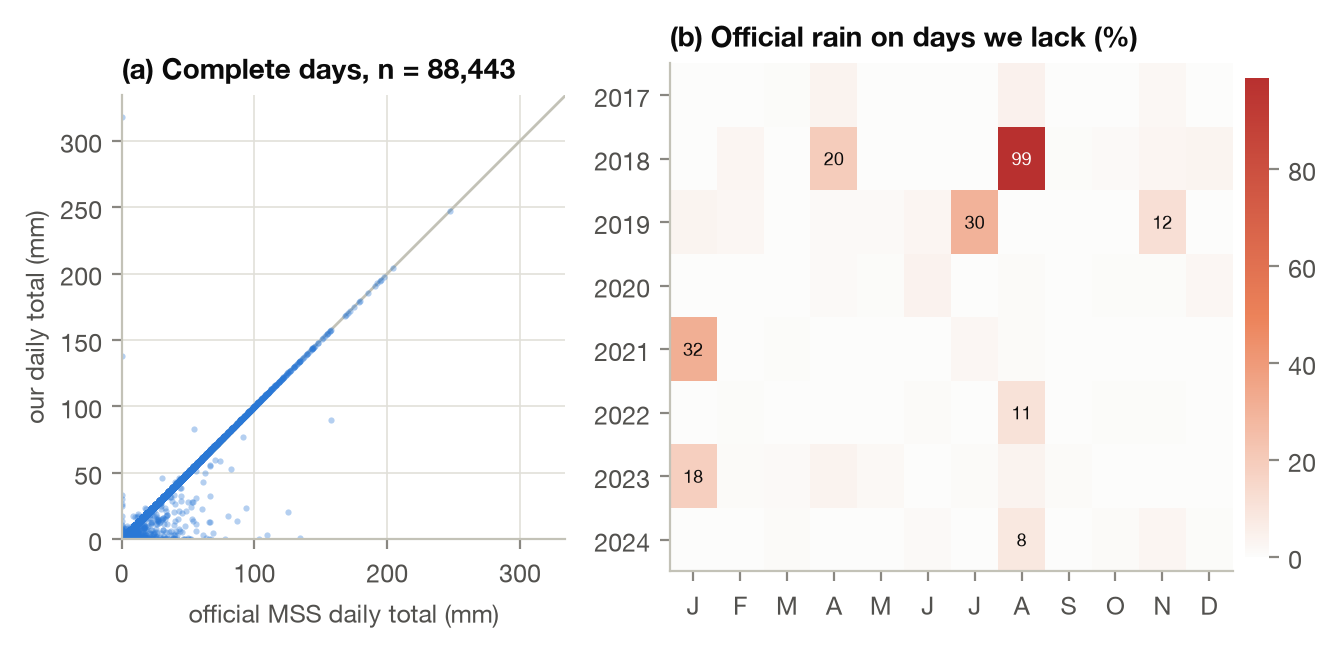
\includegraphics[width=0.9\textwidth]{fig16_mss_validation.png}
\caption{(a) Daily rain on the \val{mss_days} complete station-days, our total against the official MSS total (mm).
Nearly all points lie on the diagonal; the few far below or above it are the faulty-gauge days described in the
text. (b) Share of official rain, per year and month, that fell on days our data lack (stations reporting that month).
The losses are concentrated in a few months, above all August 2018, then January 2021 and July 2019.
\src{src/plot\_mss.py from outputs/mss/}}\label{fig:mss}
\end{figure}

% ======================================================================================================
\section{Investigating weather patterns and developing the model}
\subsection{Task 1: how we compared months and years}\label{sec:t1method}
\req{E5}
All aggregation runs in Spark (\code{src/task1.py}); only the small result tables go to Python for plotting. Because
the stations and the coverage change, the basic quantity is a \emph{rate} rather than a sum: the mean five-minute
reading over reported slots, times \val{slots_day}, that is, mm per station-day. Missing slots do not lower a month's
rate, and the number of stations in a year does not enter it. For a year we use a \emph{month-balanced} total, the sum
over the twelve months of (monthly rate $\times$ days in the month), so that a missing week in a wet month cannot
lower the year.

We split each rate into \emph{frequency}, the share of slots with rain, and \emph{intensity}, the mean rain per wet
slot in mm/h. This split is what lets us say whether a dry year had fewer showers or weaker ones. Extremes use complete
station-hours only (all twelve slots) and complete station-days (at least \val{full_day_pct}\,\% of slots). Seasons
follow the MSS monsoon calendar: north-east monsoon December--March, inter-monsoon April--May, south-west monsoon
June--September, inter-monsoon October--November.

Two checks test whether these comparisons hold. A \emph{fixed panel} of the \val{panel_n} stations that reported at
least half of every year removes the effect of stations joining and leaving the network, so a pattern that is real should appear in the panel too.
The MSS comparison of Section~\ref{sec:mss}, applied per month, finds months whose rate is distorted because the
missing days were not ordinary days.

\subsection{Task 2: target and thresholds}\label{sec:t2method}
\req{E7}\req{E8}
For station $s$, prediction time $t$ (the end of a five-minute slot) and threshold $\theta$, the label is $y=1$ if the
station's rain in $(t, t+\val{horizon}\,\text{min}]$, the sum $f_{30}$ of the next six readings, exceeds $\theta$. We
create a label only when all six future slots were reported and lie in the same calendar year as $t$. A missing
reading therefore never counts as no rain, and no label crosses a split boundary. Because $\theta$ is an input, one
model answers every threshold.

We chose the thresholds from the training years alone (Figure~\ref{fig:grid}). Wet \val{horizon}-minute totals have a
median of \val{q50}\,mm, a ninetieth percentile of \val{q90}\,mm and a ninety-ninth percentile of \val{q99}\,mm.
Measurable rain (more than \val{zero}\,mm) follows \val{f30rate.0} of prediction times, and more than
\val{grid_max}\,mm follows \val{f30rate.20}, which still gives \val{f30pos.20} cases in six years. Above that the cases
run out quickly: \val{f30pos.30} above \val{cand_th_hi1}\,mm and \val{f30pos.40} above \val{cand_th_hi2}\,mm. At the
low end, the gauge step of \val{gauge_step}\,mm makes ``more than \val{gauge_step}\,mm'' almost the same event as
``more than \val{zero}\,mm'', so we left that threshold out. The grid is therefore $\theta \in \{\val{grid}\}$\,mm,
from any measurable rain to a heavy downpour.

\begin{figure}[H]\centering
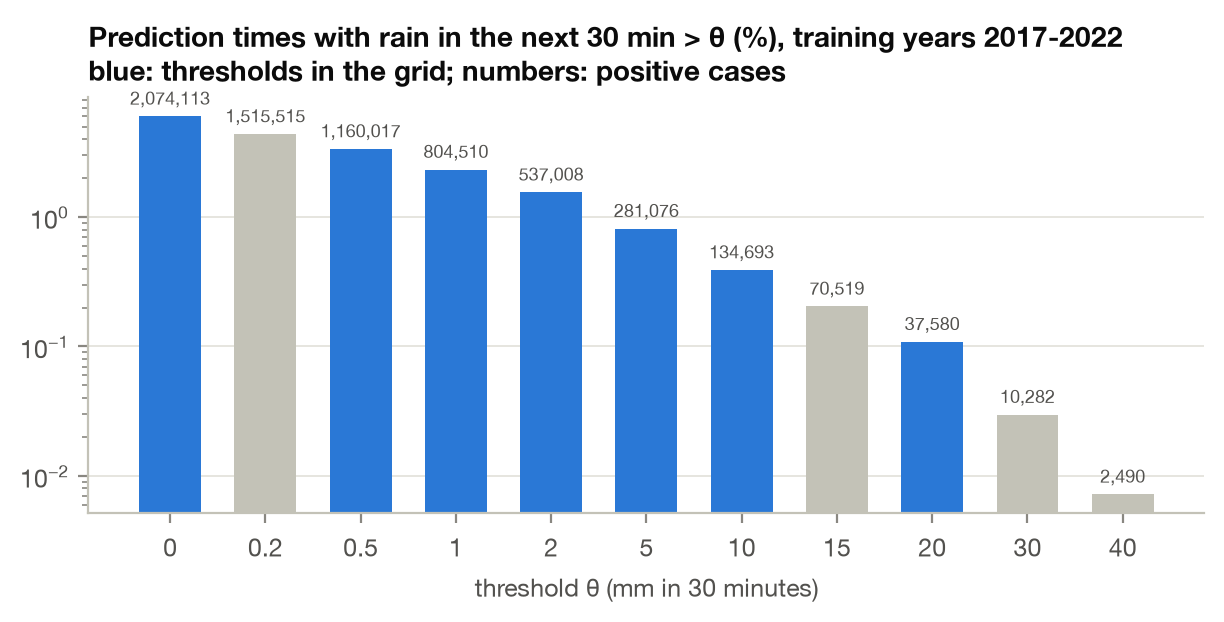
\includegraphics[width=0.75\textwidth]{fig11_threshold_grid.png}
\caption{Share of prediction times in the training years 2017--2022 followed by more than $\theta$\,mm of rain in the
next \val{horizon} minutes (log scale), with the number of positive cases above each bar. Blue bars are the thresholds
we kept. The share falls steeply with $\theta$, and beyond \val{grid_max}\,mm few cases remain.
\src{src/plot\_task2.py from src/task2\_features.py}}\label{fig:grid}
\end{figure}

\subsection{Task 2: features}
The brief says the model should take the station, prediction time and threshold as inputs, but not whether it may also
look at observations available at the prediction time. We built both readings behind the same interface,
$\text{predict}(s,t,\theta)$ in \code{src/predict.py}, and report both.

\emph{Model A} (strict) uses only functions of the three inputs, which makes it climatology learned by MLlib:
\begin{itemize}
\item the station: one-hot index, coordinates, and its wet-slot rate in the training years;
\item the time: time of day and day of year as sine/cosine pairs, so that the end of a day sits next to the start of
the next, plus month, hour and monsoon season;
\item the threshold: $\theta$, $\log(1+\theta)$ and a one-hot $\theta$ class.
\end{itemize}
\emph{Model B} (nowcast) keeps all of A's features and, inside $\text{predict}$, also looks up what was observed up to
$t$:
\begin{itemize}
\item the station's own rain in the last \val{win_list}, the minutes since its last wet slot, and how many of the
last \val{win_slots} slots were reported;
\item at the same slot, the maximum, mean and share wet of the \val{k_nb} nearest stations;
\item the island-wide share of wet stations, and the maximum and mean \val{horizon}-minute totals;
\item the difference between the rain of the last \val{horizon} minutes and $\theta$.
\end{itemize}
Every B feature uses only readings whose slot ends at or before $t$. We computed them with Spark window functions over
each station's readings ordered by slot, using \code{rangeBetween} on the slot index so that a missing slot is simply
absent from the window instead of shifting it (\code{src/task2\_features.py}).

\subsection{Task 2: model, split and evaluation}\label{sec:t2model}
\req{E9}
We split by time: training on 2017--2022, model choice on 2023, and a single test on 2024. A random split (the
\code{randomSplit} of Lecture 6) would put neighbouring five-minute rows of the same storm into both training and test
and so overstate the test score.

Before fitting any model we froze the evaluation plan. The split, threshold grid, sampling, features, candidate models,
metrics, baselines and selection rule are written in \code{config/eval\_plan.json}, and we recorded the file's SHA-256
hash (\code{\val{plan_sha}\ldots}) at \val{plan_frozen}. The training and test scripts refuse to run if the file has
changed since then, and the test script refuses to run a second time (\code{checks/eval\_plan.py}). No result on 2024
could therefore feed back into a modelling choice.

Most prediction times are followed by no rain at all (Figure~\ref{fig:grid}), so we sample them. The sample is
deterministic, drawn by a hash of station, slot and seed, and has two strata: \emph{active} times, with rain at the
station in the last \val{active_hours} hours or the next \val{horizon} minutes, are sampled at rate
\val{rate_active.train} in training, and the rest at \val{rate_inactive.train}. Every row is weighted by the inverse of
its sampling rate, in fitting and in every metric, so all results refer to all prediction times and not only to the
sample. Each training row is paired with one $\theta$ from the grid, while each validation and test row is scored at
every $\theta$. This gives \val{n_train} training rows, \val{n_validation} validation rows and \val{n_test} test rows.

Each candidate is an MLlib \code{Pipeline}: \code{SQLTransformer} for the derived inputs, \code{StringIndexer} for the
station, \code{OneHotEncoder} and \code{VectorAssembler}, and then \code{LogisticRegression} or \code{GBTClassifier}
fitted with \code{weightCol}. The saved \code{PipelineModel} therefore takes the raw columns. For each of A and B the
candidates were logistic regression at two regularisation strengths and gradient-boosted trees, and the plan fixed the
selection rule in advance: the lowest weighted log loss on 2023, pooled over the grid.

We compare the models with two baselines, both estimated on the full, unsampled training years. \emph{Climatology} is
the frequency of $y$ per (station, month, hour, $\theta$), shrunk toward the (month, hour, $\theta$) frequency with
\val{clim_pseudo} pseudo-counts. \emph{Persistence} is the frequency of $y$ given whether the last \val{horizon}
minutes at the station exceeded $\theta$.

AUC-ROC and AUC-PR come from MLlib's \code{BinaryClassificationEvaluator}, with \code{weightCol}. The other metrics
are Spark aggregations: Brier score, Brier skill against the base rate, log loss and a \val{rel_bins}-bin reliability
table. We report every metric pooled over the grid and per $\theta$. We also count how often the predicted probability
\emph{rises} with $\theta$, which should never happen, since a higher threshold is a rarer event. We read AUC-PR first
because the events are rare: a model with no skill scores the base rate, not one half.

% ======================================================================================================
\section{Computing environment}
\req{E10}\req{E2}
\subsection{Local machine}
All reported numbers were computed on our local machine. Every Spark job writes an \code{env.json} file when it starts
(\code{checks/env\_capture.py}); the specification below and Table~\ref{tab:env} are read from those files.

\val{env.cpu} with \val{env.ncpu} logical CPUs and \val{env.ram}\,GiB of memory, running \val{env.os}. Apache Spark
\val{env.spark} (PySpark) on Java \val{env.java} and Python \val{env.python}, in local mode, master
\code{\val{env.master}}: one JVM whose driver runs \val{env.parallelism} task threads, one per logical CPU, with
driver memory \val{env.driver_mem}, \val{env.shuffle} shuffle partitions and session time zone Asia/Singapore. In
local mode the driver also does the executors' work, so the driver memory is the memory Spark has. The recorded stages
took about \val{env.total_min} minutes of wall time in total.

\begin{table}[H]\centering\small
\begin{tabular}{llr}
\toprule
Stage & Run id (\texttt{runs/<id>/env.json}) & Wall time (s) \\
\midrule
ingest (CSV $\to$ Parquet) & 20261017T152317-ingest & 23 \\
ingest check & 20261017T152343-ingest\_check & 19 \\
cleaning + ledger & 20261017T152406-clean & 625 \\
ledger check & 20261017T153435-clean\_ledger & 14 \\
coverage & 20261017T153452-coverage\_check & 4 \\
stuck-gauge check & 20261017T153458-stuck\_runs & 11 \\
Task 1 aggregation & 20261017T153512-task1 & 63 \\
Task 2 features & 20261017T153619-task2\_features & 103 \\
Task 2 samples + baselines & 20261017T153805-task2\_sample & 42 \\
Task 2 fit + validation & 20261017T143824-task2\_train & not recorded$^{\dagger}$ \\
Task 2 test (once) & 20261017T150558-task2\_test & 83 \\
MSS validation & 20261017T154130-mss\_validate & 61 \\
\bottomrule
\end{tabular}

\caption{Local runs behind the reported outputs: one row per pipeline stage, with the run identifier (its
\code{runs/<id>/env.json} holds the full environment) and wall time in seconds. Of the recorded stages, cleaning takes
the longest. $^\dagger$ The fit-and-validation run started before we added wall-time capture; its per-model fit times
are in Table~\ref{tab:val}. \src{src/report\_macros.py from runs/*/env.json}}\label{tab:env}
\end{table}

\subsection{Google Cloud Dataproc}
We also ran the pipeline once on Google Cloud Dataproc, from ingestion to the Task 2 fit and validation. The 2024 test and every number reported elsewhere come from the local runs. Cluster \code{dsa5208-p2}, zone \code{asia-southeast1-c}, image \code{3.0.3-debian13}: 1 n2-standard-4 master and 2 n2-standard-4 workers, each with a boot disk of 80\,GB pd-balanced; Spark 4.1.2 on Java 21.0.12.1 and Python 3.12.13, master \code{yarn}; 2 executors with 3 cores and 8g each, driver memory 8g, 48 shuffle partitions, dynamic allocation off.

These three machines took the project's whole vCPU quota, so the cluster could not be larger. We sized the executors as Lecture 6 does. Each machine has 4 vCPUs and 16\,GiB of memory. Lecture 6 recommends three to five cores per executor and keeping some capacity on each worker for the cluster manager and the operating system, so we ran one executor per worker with 3 cores and left the remaining vCPU free. Executor memory, plus an overhead that Lecture 6 puts at about a tenth of it (more for PySpark), has to fit within what YARN offers on a worker, which is less than the machine's 16\,GiB; 8g fits with room to spare for the Python worker processes. We turned dynamic allocation off so that every job ran on exactly these executors. The raw CSVs were downloaded from data.gov.sg straight into Cloud Storage by a job on the cluster (\code{cloud/fetch\_raw\_on\_cluster.py}) rather than uploaded from our local machine. The run used two clusters of this configuration. The stages up to the cleaning-ledger check ran on the first (\code{cloud\_run/cluster\_part1.json}). A status call on our side hung, the cluster sat idle until its idle limit deleted it, and we resumed the remaining stages on a second cluster, which read the first cluster's outputs from the same Cloud Storage prefix.

Table~\ref{tab:cloudcmp} compares the wall time of each stage; the cloud stages took about 44 minutes in total. Every Dataproc job pays a fixed start-up cost (the trivial environment-check job took 29\,s), and on the short stages that cost dominates. Our local machine also has 10 cores against the cluster's 6 executor cores, and reads local disk rather than Cloud Storage. Cleaning, the longest data stage, is where the cluster catches up.

To check that the cluster computed the same results, \code{checks/cloud\_parity.py} compares its outputs with the local ones (22 tables). Counts that do not depend on the order of summation (rows, stations, every cleaning rule, coverage, slot and event counts, sample sizes) match exactly; across 34 floating-point columns the largest relative difference is $3.1\times10^{-13}$. The 4 threshold counts on summed rain (hours with at least 20 or 40\,mm, days with at least 50\,mm) differ by at most 4 per row. Most readings are multiples of 0.2\,mm, so many totals equal a threshold exactly, and a floating-point sum lands just above or below it depending on the order in which Spark adds partitions. \code{checks/threshold\_boundary.py} counts the totals within $10^{-6}$\,mm of each threshold, and all differences are within that count. The 5 approximate quantiles (Spark's \code{percentile\_approx}) differ by up to 1.3\,\%. On 2023 the Task 2 fit on the cluster chose the same models as the local fit; Model B's validation AUC-PR is 0.6677 on Dataproc and 0.6677 locally, and the largest AUC-PR difference over all candidates is 0.0023.

\begin{table}[H]\centering\small
\begin{tabular}{lrrr}
\toprule
Stage & Local (s) & Dataproc (s) & Dataproc / local \\
\midrule
ingest (CSV $\to$ Parquet) & 23 & 156 & 6.7 \\
ingest check & 19 & 45 & 2.3 \\
cleaning + ledger & 625 & 580 & 0.9 \\
ledger check & 14 & 48 & 3.4 \\
coverage & 4 & 51 & 13.4 \\
Task 1 aggregation & 63 & 143 & 2.3 \\
Task 2 features & 103 & 255 & 2.5 \\
Task 2 samples + baselines & 42 & 133 & 3.2 \\
Task 2 fit + validation & not recorded & 1251 & -- \\
\bottomrule
\end{tabular}

\caption{Wall time per stage in seconds, on the local machine and on Dataproc, and their ratio; a ratio below one means Dataproc was faster. \src{src/report\_macros.py from runs/*/env.json and cloud\_run/job\_times.json (Dataproc jobs API; driver start to exit, including the small Cloud Storage copies)}}\label{tab:cloudcmp}
\end{table}


% ======================================================================================================
\section{Results}
\subsection{Task 1: patterns within a year}
\req{E4}\req{E6}
The year has two wet peaks and two dry spells (Figures~\ref{fig:month} and~\ref{fig:doy}). Over 2017--2024,
\val{wettest_month} is the wettest month at \val{wettest_month_rate}\,mm per station-day and \val{driest_month} the
driest at \val{driest_month_rate}. After November come December (\val{mrate.Dec}), April (\val{mrate.Apr}) and
January (\val{mrate.Jan}); February (\val{mrate.Feb}) and July--August (\val{mrate.Jul}, \val{mrate.Aug}) are the dry
spells. Grouped by monsoon season, the October--November inter-monsoon is the wettest at \val{season_rate.imii}\,mm/day
and the south-west monsoon the driest at \val{season_rate.sw}, with the north-east monsoon (\val{season_rate.ne}) and
the April--May inter-monsoon (\val{season_rate.imi}) in between. These are eight-year means, and single years scatter
widely around them: the same month can be three times as wet in one year as in another.

\begin{figure}[H]\centering
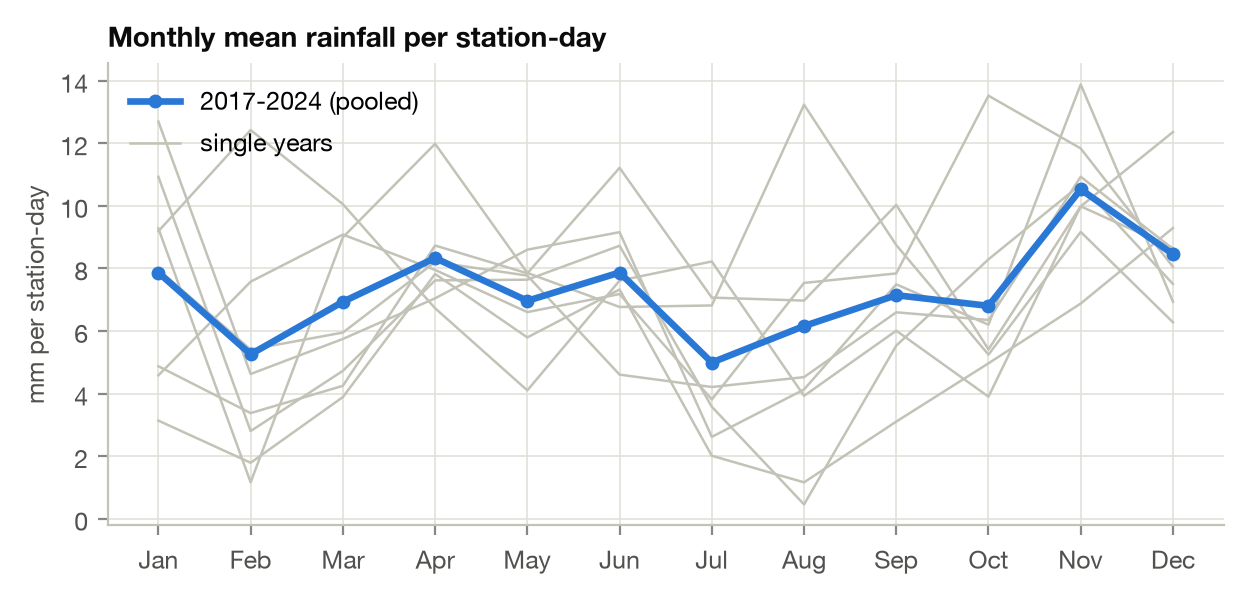
\includegraphics[width=0.66\textwidth]{fig02_monthly_cycle.png}
\caption{Mean rainfall per station-day (mm) in each calendar month, pooled over 2017--2024 (blue) and for each single
year (grey). The pooled cycle peaks in November and April and dips in February and July; single years spread far more
widely than the pooled months differ from each other. \src{src/plot\_task1.py from src/task1.py}}\label{fig:month}
\end{figure}
\begin{figure}[H]\centering
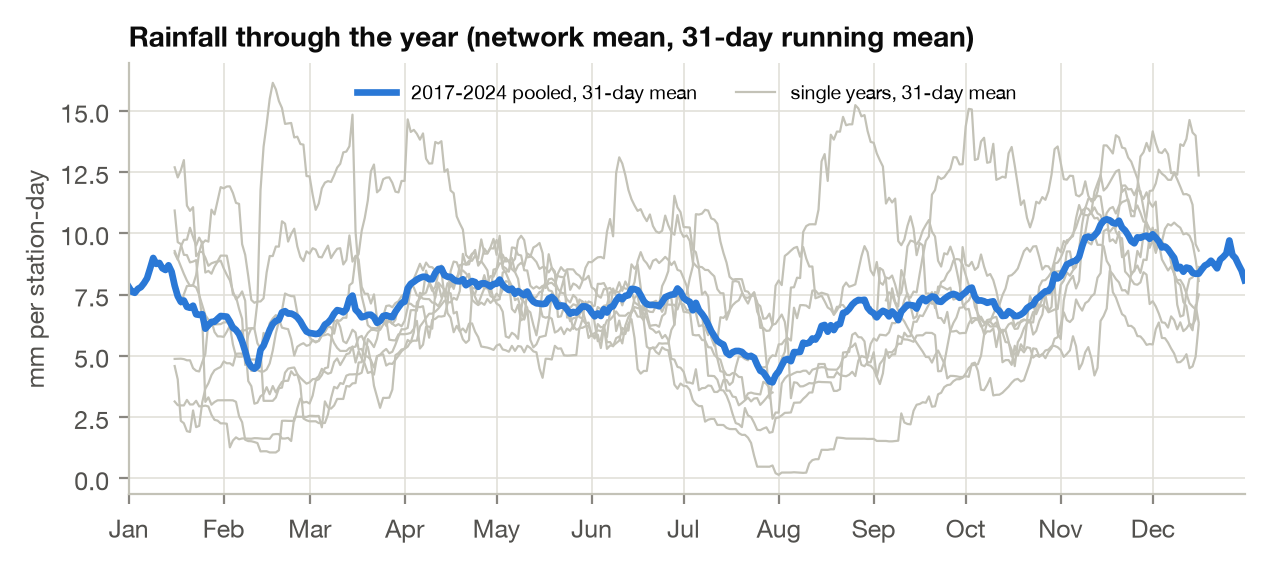
\includegraphics[width=0.66\textwidth]{fig10_day_of_year.png}
\caption{Network rainfall (mm per station-day) through the calendar year as a \val{smooth_days}-day running mean (total
rain over reported slots in the window), pooled over 2017--2024 (blue) and for each year (grey). The two dry spells
fall in mid-February and around the turn of July and August. \src{src/plot\_task1.py from src/task1.py}}\label{fig:doy}
\end{figure}

Within the day, the timing depends on the season (Figure~\ref{fig:diurnal}). In the north-east monsoon and both
inter-monsoons, rain peaks in the mid-afternoon, at \val{peak_hour.ne}, \val{peak_hour.imi} and \val{peak_hour.imii}
SGT respectively, with the highest rate (\val{peak_rate.imii}\,mm/h) in October--November. Overnight the rate falls to
about \val{min_rate.ne}\,mm/h. We read this as convective storms building over land in the afternoon heat. The
south-west monsoon peaks instead at \val{peak_hour.sw} (\val{peak_rate.sw}\,mm/h, against \val{min_rate.sw} at its
lowest hour), when squall lines that form over
Sumatra overnight reach Singapore. Over all seasons, \val{share_12_20} of the rain falls between \val{share_win_lo} and
\val{share_win_hi}.

\begin{figure}[H]\centering
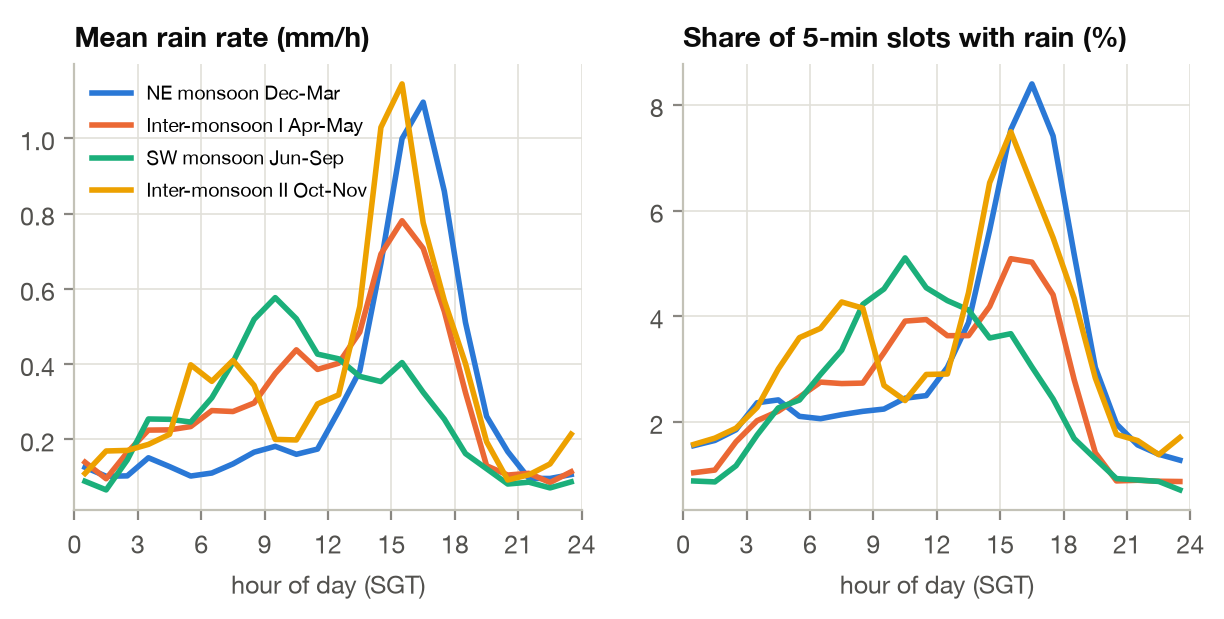
\includegraphics[width=0.8\textwidth]{fig05_diurnal_by_season.png}
\caption{Rain by hour of day (SGT) in each monsoon season, 2017--2024: mean rate in mm/h (left) and share of
five-minute slots with rain (right). Three seasons peak in the mid-afternoon; the south-west monsoon (green) peaks at
\val{peak_hour.sw} instead. \src{src/plot\_task1.py from src/task1.py}}\label{fig:diurnal}
\end{figure}

A month's rate is the frequency of rain times its intensity, and the two wet peaks are built differently
(Figure~\ref{fig:freqint}). Over the whole period it rains in only \val{wet_pct_all}\,\% of slots, yet
\val{intense_share_all} of all rain falls at \val{intense_mmh}\,mm/h or more. January departs from this in one
direction: it has the most wet slots (\val{wetpct.Jan}\,\%) but the gentlest rain, \val{intmon.Jan}\,mm/h when wet,
and only \val{intshare.Jan} of its rain falls at \val{intense_mmh}\,mm/h or more. That is long, steady monsoon rain.
April departs in the other: its wet slots are close to the all-period share (\val{wetpct.Apr}\,\%), but it has the
hardest rain (\val{intmon.Apr}\,mm/h, with \val{intshare.Apr} of it at \val{intense_mmh}\,mm/h or more), which points
to short thunderstorms.

\begin{figure}[H]\centering
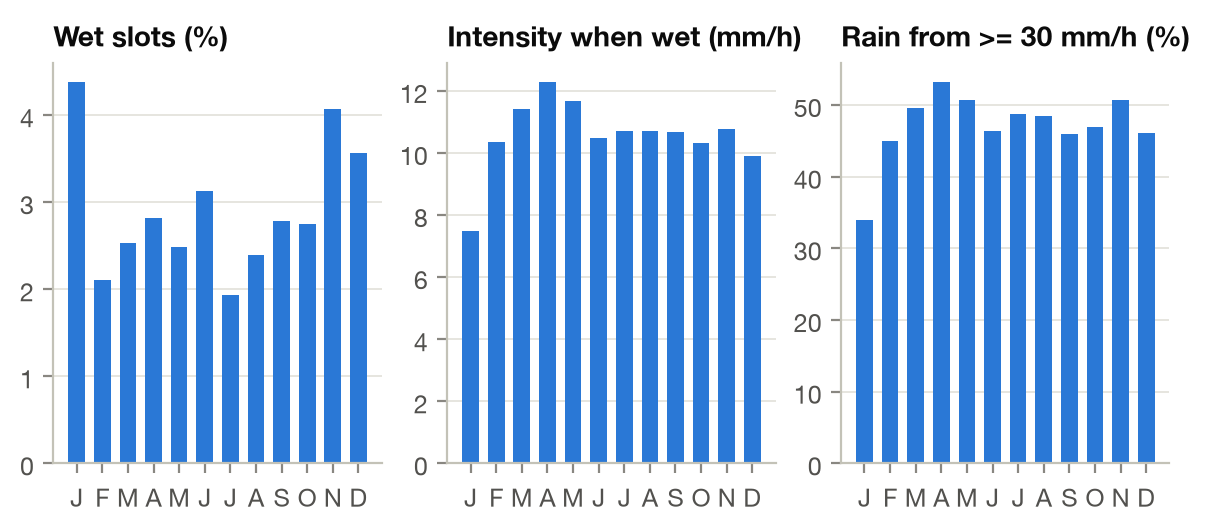
\includegraphics[width=0.85\textwidth]{fig06_frequency_intensity_month.png}
\caption{Each calendar month, 2017--2024: share of five-minute slots with rain (\%), mean intensity of wet slots
(mm/h), and share of the month's rain that fell in slots of at least \val{intense_mmh}\,mm/h (\%). January is wet most
often but most gently; April has the hardest rain. \src{src/plot\_task1.py from src/task1.py}}\label{fig:freqint}
\end{figure}

Across the island, stations further west tend to be wetter, in every season (Figure~\ref{fig:map}). The correlation of
a station's mean rate with its longitude is \val{corr_lon.ne} in the north-east monsoon and \val{corr_lon.sw} in the
south-west monsoon, the season whose squalls arrive from the west. Over the \val{n_st_1yr} stations with at least a
year of data, the mean rate runs from \val{st_rate_min}\,mm/day at \val{st_rate_min_id} to \val{st_rate_max}\,mm/day
at \val{st_rate_max_id}.

\begin{figure}[H]\centering
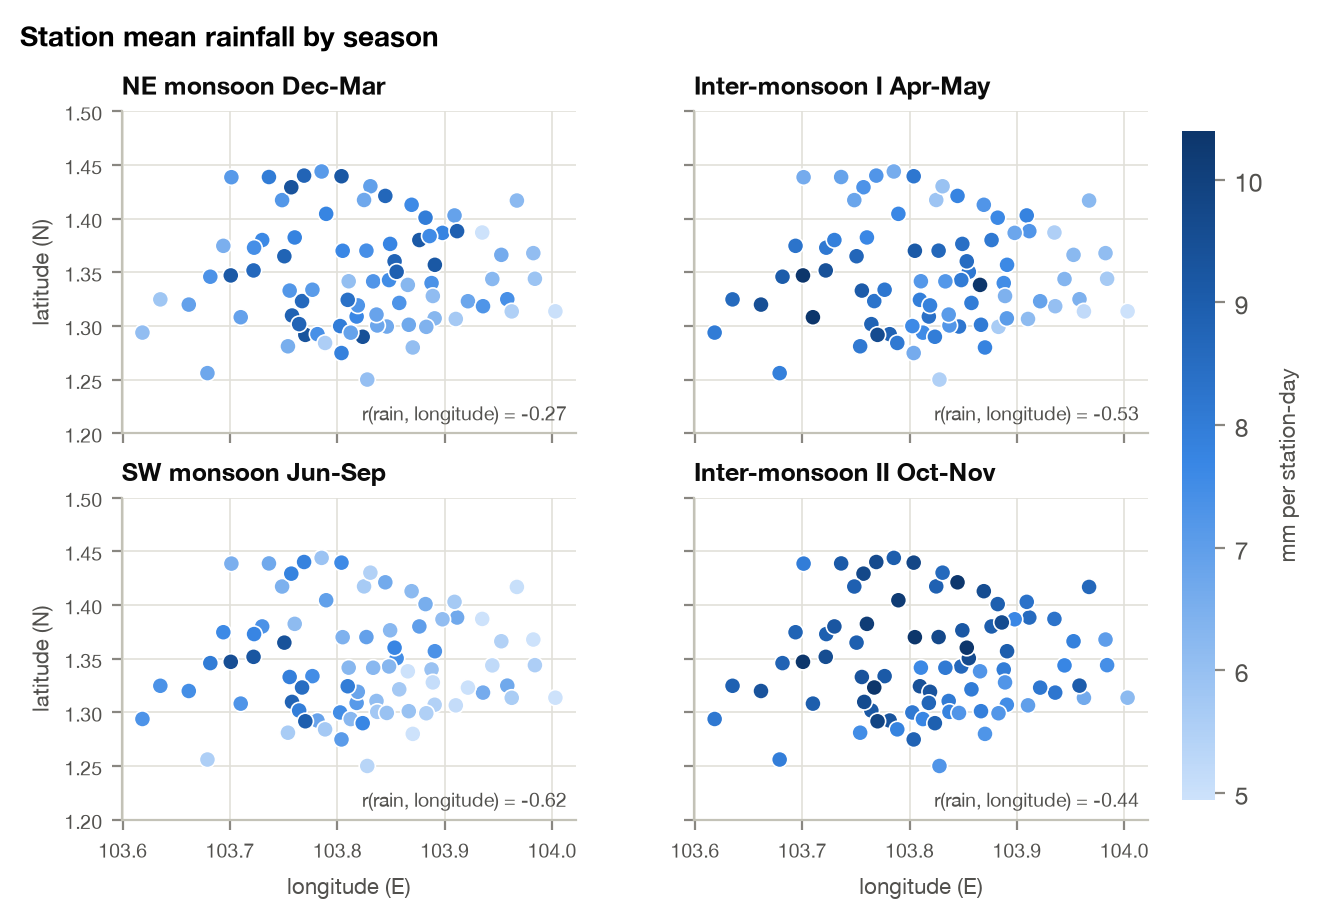
\includegraphics[width=0.68\textwidth]{fig09_station_map_season.png}
\caption{Mean rainfall per station-day (mm) at each station by monsoon season, 2017--2024; $r$ is the correlation of
the station's rate with its longitude. The west--east gradient is strongest in the south-west monsoon. \src{src/plot\_task1.py from src/task1.py}}\label{fig:map}
\end{figure}

\subsection{Task 1: changes across 2017--2024}
\req{E5}
Month-balanced annual rainfall per station (Figure~\ref{fig:annual}) was lowest in 2019 (\val{ann.2019}\,mm) and
highest in 2021 and 2022 (\val{ann.2021} and \val{ann.2022}\,mm), against a 2017--2024 mean of \val{ann_mean}\,mm. We
balance by month and divide by station because a plain network sum exaggerates the change. It puts 2021 at
\val{naive_ratio_21_17} times 2017; per station the ratio is \val{bal_ratio_21_17}. The difference is that more
stations reported in 2021. Restricting the calculation to the fixed panel of \val{panel_n} stations that reported in
every year changes no annual total by more than \val{panel_maxdev}, so changes in which stations reported do not
explain these totals.

Year-to-year differences follow how often it rained much more than how hard. Across the eight years, the annual total
correlates at \val{corr_freq} with the frequency of rain and at \val{corr_int} with its intensity. In 2019 the
frequency index fell to \val{freqidx.2019} (2017--2024 mean = \val{index_base}) while intensity stayed at
\val{intidx.2019}. From 2020 on, frequency stayed above the mean, reaching \val{freqidx.2023} in 2023.

\begin{figure}[H]\centering
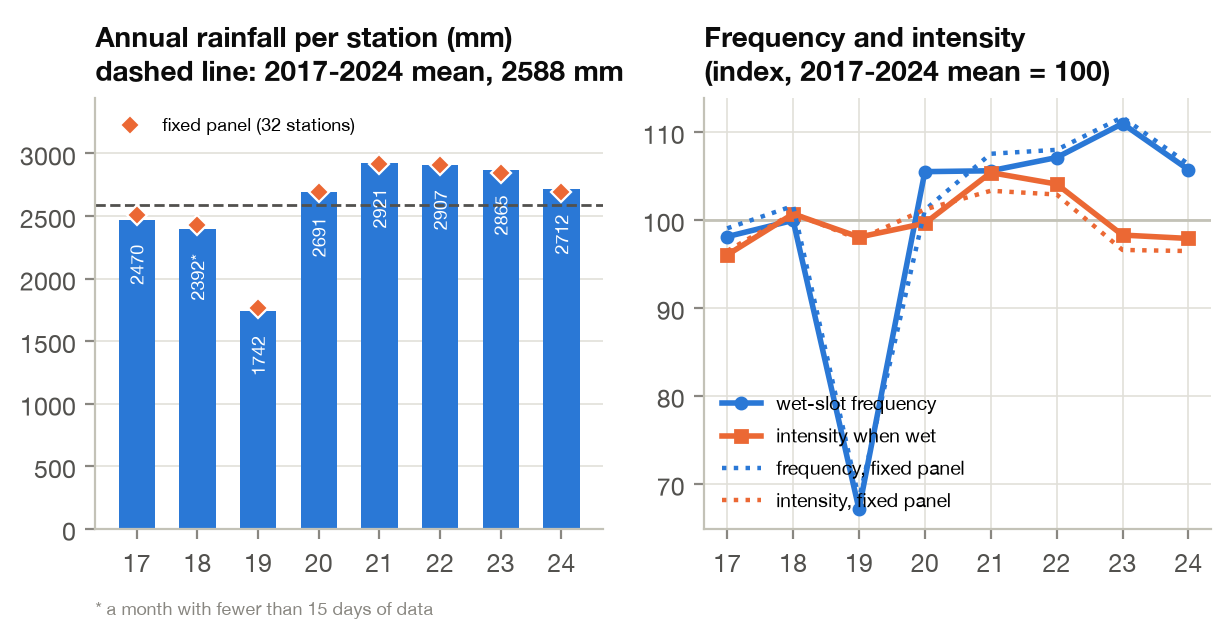
\includegraphics[width=0.85\textwidth]{fig04_annual_balanced.png}
\caption{Left: month-balanced annual rainfall per station (mm), 2017--2024, for all stations (bars) and the fixed panel
of \val{panel_n} stations (diamonds). Right: frequency of wet slots and intensity when wet, as indices with the
2017--2024 mean at \val{index_base}, for all stations (solid) and the fixed panel (dotted). The 2019 dip is a drop in
frequency, not intensity, and the panel tracks the full network in every year. \src{src/plot\_task1.py from src/task1.py}}\label{fig:annual}
\end{figure}

The seasonal anomalies (Figure~\ref{fig:season}) show which part of the year made each year wet or dry. In 2019 every
season was dry, the south-west monsoon most of all (\val{sanom.sw.2019}\,\%). The south-west monsoons of 2020 and 2021
were wet (\val{sanom.sw.2020}\,\% and \val{sanom.sw.2021}\,\%), as were the October--November inter-monsoon of 2022
(\val{sanom.imii.2022}\,\%) and the north-east monsoon of 2023 (\val{sanom.ne.2023}\,\%). Single months
(Figure~\ref{fig:anom}) swing much more, and some of those cells are distorted by gaps
(Section~\ref{sec:gapmonths}).

\begin{figure}[H]\centering
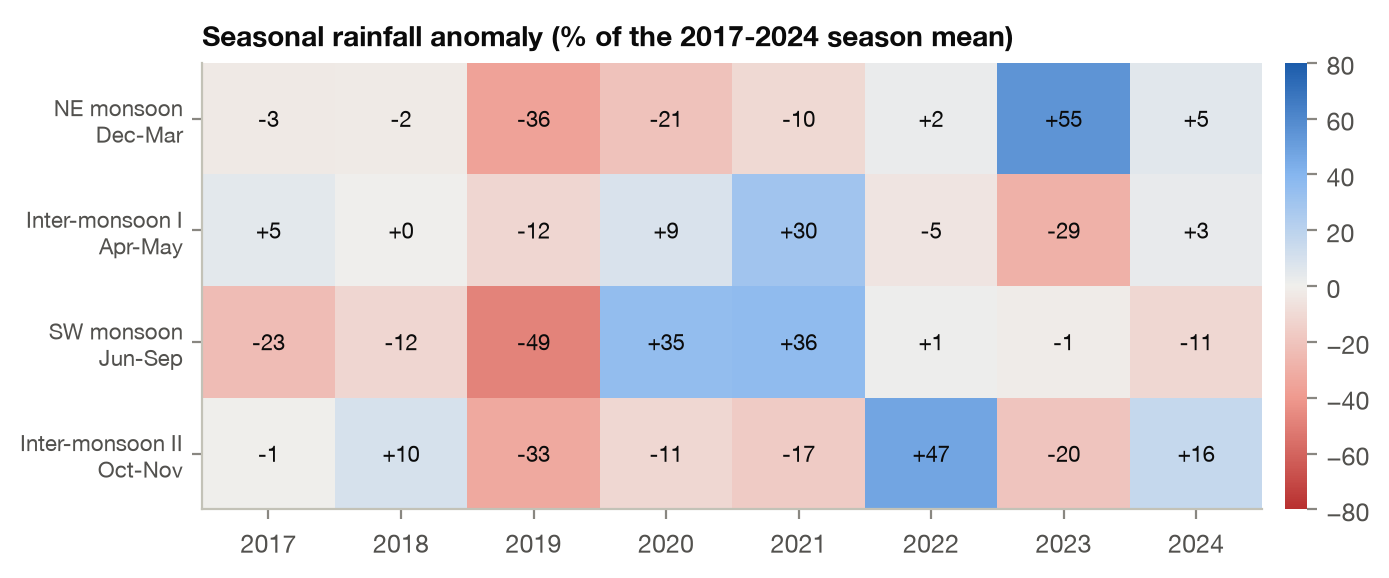
\includegraphics[width=0.72\textwidth]{fig08_season_anomaly.png}
\caption{Seasonal rainfall anomaly for each year 2017--2024, as \% of the 2017--2024 mean for that season (blue wetter,
red drier). 2019 is dry in all four seasons; the largest wet anomaly is the 2023 north-east monsoon. \src{src/plot\_task1.py from src/task1.py}}\label{fig:season}
\end{figure}
\begin{figure}[H]\centering
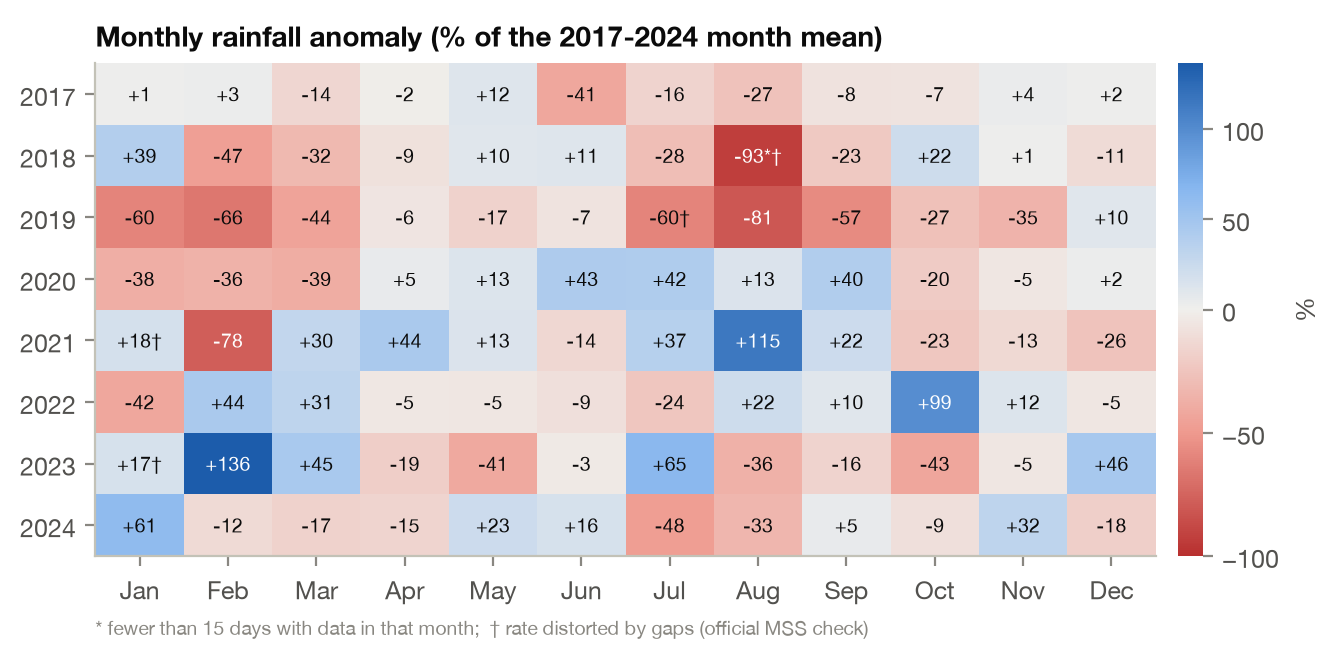
\includegraphics[width=0.8\textwidth]{fig03_year_month_anomaly.png}
\caption{Monthly rainfall anomaly for each year 2017--2024, as \% of the 2017--2024 mean for that calendar month.
* fewer than \val{low_cov_days} days of data; $\dagger$ the comparison with official MSS records finds our rate
distorted by gaps (Table~\ref{tab:gapmonths}). The marked cells should not be read at face value. \src{src/plot\_task1.py from src/task1.py and src/mss\_validate.py}}\label{fig:anom}
\end{figure}

Heavy rain was rarest in 2019 and most frequent in 2021 and 2022 (Figure~\ref{fig:ext}). Hours with at least
\val{heavy_hour_mm}\,mm numbered \val{heavyh.2019} per \val{per_hours} complete station-hours in 2019, against
\val{heavyh.2017} in 2017 and \val{heavyh.2018} in 2018, and \val{heavyh.2022} in 2022. Days with at least
\val{heavy_day_mm}\,mm numbered \val{heavyd.2019} per \val{per_days} complete station-days in 2019, against
\val{heavyd.2017} and \val{heavyd.2018} in the two years before, and \val{heavyd.2021} in 2021. Across stations, the median of each station's annual
maximum hour rose from \val{medmaxhour.2017}\,mm in 2017 to \val{medmaxhour.2022}\,mm in 2022, and the largest single
hour in the data (\val{maxhour.2022}\,mm) fell in 2022. The official MSS records show the same jump on the days both
sources cover completely: \val{mss_heavyrate_off.2019} heavy days per \val{per_days} matched station-days in 2019 and
\val{mss_heavyrate_off.2021} in 2021 (ours: \val{mss_heavyrate_ours.2019} and \val{mss_heavyrate_ours.2021}), so it is
not an artefact of our data. We do not call it a trend. Eight years is a short record, and the years with the most
heavy rain were also the wettest overall.

\begin{figure}[H]\centering
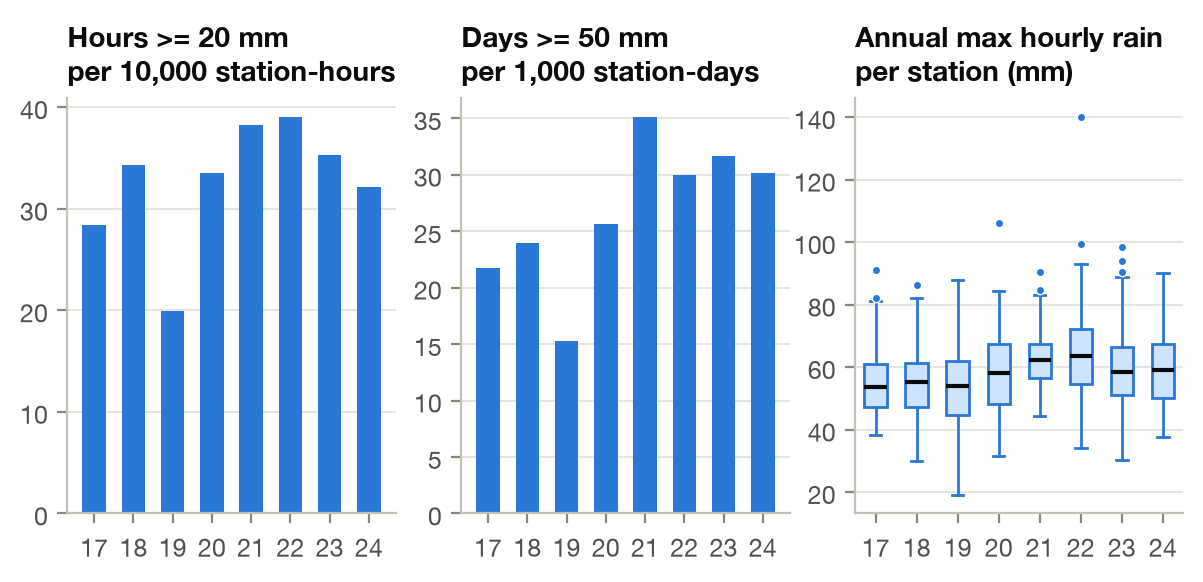
\includegraphics[width=0.85\textwidth]{fig07_extremes_by_year.png}
\caption{Rain extremes by year, 2017--2024: hours with at least \val{heavy_hour_mm}\,mm per \val{per_hours} complete
station-hours (left), days with at least \val{heavy_day_mm}\,mm per \val{per_days} complete station-days (middle), and
the spread across stations of each station's largest hourly total (right). Both counts are lowest in 2019 and highest
in 2021--2022. \src{src/plot\_task1.py from src/task1.py}}\label{fig:ext}
\end{figure}

\subsection{Task 1: months that the gaps distort}\label{sec:gapmonths}
A rate computed over reported slots is unbiased only if the missing days are like the reported ones. To find the
months where they are not, we compared each year-month's rate with the official MSS rate on the same station-months
(Table~\ref{tab:gapmonths}). In most months the two agree (median ratio \val{mss_month_median_ratio}). Where they
disagree, the month has large gaps.

January 2021 is the clearest case. Figure~\ref{fig:anom} shows it only \val{manom.2021.Jan}\,\% above an average
January, yet MSS reported it as Singapore's wettest January on record. On the same stations the official rate is
\val{mssoff.2021.Jan}\,mm/day against our \val{mssours.2021.Jan} (ratio \val{mssratio.2021.Jan}). The network was down on
\val{jan21_gap_days} (from \val{jan21_last} on \val{jan21_last_day}), and those were the wettest days of the month.
Measured against our average January, the official figure would be \val{mssoffanom.2021.Jan}\,\%. Our 2021 annual
total (\val{ann.2021}\,mm) is too low for the same reason.

August 2018, with data on only \val{days.2018.aug} days, shows as \val{manom.2018.Aug}\,\% in Figure~\ref{fig:anom}.
That is the gap, not the weather: on the same stations the official rate is \val{mssoff.2018.Aug}\,mm/day against our
\val{mssours.2018.Aug}.

January 2023 is distorted the other way. With \val{days.2023.jan} days of data network-wide, our rate is
\val{mssratio.2023.Jan} times the official one on the same station-months, because the days we lack were drier than the
days we have. Figure~\ref{fig:anom} therefore shows the month as wetter than usual (\val{manom.2023.Jan}\,\%), while
officially it was drier (\val{mssoffanom.2023.Jan}\,\%). Changi (S24) is missing for most of the month
(Table~\ref{tab:gaps}).

The two rates also differ by more than \val{gap_ratio_pct}\,\% in \val{mss_odd_n} months without a large gap:
\val{mss_odd_list}. Partial days and the different spread of the two networks over the island are the likely causes.
The fixed-panel check covers the annual totals and the frequency and intensity indices; any claim about a single
month should be read together with Table~\ref{tab:gapmonths}.

\begin{table}[H]\centering\small
\begin{tabular}{lrrrrr}
\toprule
Month & Ours (mm/day) & Official (mm/day) & Ratio & Official rain on days we lack & Our anomaly (\%) \\
\midrule
Aug 2018 & 0.46 & 2.92 & 0.16 & 99\,\% & $-$93 \\
Jan 2021 & 9.18 & 13.38 & 0.69 & 32\,\% & $+$18 \\
Jul 2019 & 1.99 & 2.38 & 0.84 & 30\,\% & $-$60 \\
Jan 2023 & 9.11 & 7.30 & 1.25 & 18\,\% & $+$17 \\
\bottomrule
\end{tabular}

\caption{Months whose rate differs by more than \val{gap_ratio_pct}\,\% from the official rate on the same
station-months while more than \val{gap_missed_pct}\,\% of the official rain fell on days we lack. A ratio below one
means our rate is too low. \src{src/mss\_validate.py}}\label{tab:gapmonths}
\end{table}

\subsection{Task 2: model choice on 2023}
\req{E9}
Table~\ref{tab:val} gives every candidate and both baselines on the validation year, pooled over the threshold grid
(base rate \val{val_base}).

\begin{table}[H]\centering\scriptsize
\resizebox{\textwidth}{!}{\begin{tabular}{lrrrrrrrr}
\toprule
Model (validation 2023) & AUC-ROC & AUC-PR & Brier & BSS & Log loss & Mean $p$ & $p$ rises with $\theta$ & Fit (s) \\
\midrule
Climatology baseline & 0.788 & 0.094 & 0.02165 & 0.037 & 0.0995 & 0.0211 & 0.00\,\% & -- \\
Persistence baseline & 0.868 & 0.422 & 0.01528 & 0.321 & 0.0682 & 0.0220 & 0.00\,\% & -- \\
A: logistic regression (reg 0.0001) & 0.797 & 0.082 & 0.02175 & 0.033 & 0.0960 & 0.0210 & 0.00\,\% & 6 \\
A: logistic regression (chosen) & 0.797 & 0.085 & 0.02174 & 0.033 & 0.0959 & 0.0211 & 0.00\,\% & 6 \\
A: gradient-boosted trees (depth 5, trees 60) & 0.808 & 0.098 & 0.02179 & 0.031 & 0.1007 & 0.0325 & 0.04\,\% & 121 \\
B: logistic regression (chosen) & 0.963 & 0.668 & 0.01204 & 0.465 & 0.0477 & 0.0228 & 0.00\,\% & 15 \\
B: logistic regression (reg 0.001) & 0.964 & 0.663 & 0.01214 & 0.460 & 0.0479 & 0.0228 & 0.00\,\% & 12 \\
B: gradient-boosted trees (depth 5, trees 80) & 0.978 & 0.728 & 0.01100 & 0.511 & 0.0510 & 0.0352 & 0.66\,\% & 167 \\
B: gradient-boosted trees (depth 7, trees 80) & 0.980 & 0.732 & 0.01092 & 0.514 & 0.0506 & 0.0358 & 1.57\,\% & 286 \\
\bottomrule
\end{tabular}
}
\caption{Validation year 2023: every candidate and both baselines, weighted, pooled over $\theta$. BSS: Brier skill
score against the base rate. ``$p$ rises with $\theta$'': share of adjacent-$\theta$ pairs where the predicted
probability goes up, which should never happen. The selection rule takes the lowest log loss. \src{src/task2\_train.py}}\label{tab:val}
\end{table}

The two baselines are simple rules. Climatology predicts the training-years frequency of the event for that
station, month and hour; persistence assumes the last half hour repeats. Model A is no better than climatology: AUC-PR
\val{v.A.all.aucpr} against \val{v.clim.all.aucpr}, and Brier skill \val{v.A.all.bss} against \val{v.clim.all.bss}.
Given only the station, the time and $\theta$, the best possible answer is the climatological frequency, and MLlib
learns roughly that. Model B is well ahead of both baselines. Its AUC-PR is \val{v.B.all.aucpr}, against
\val{v.pers.all.aucpr} for persistence and \val{v.clim.all.aucpr} for climatology, and its Brier skill
\val{v.B.all.bss}, against \val{v.pers.all.bss} and \val{v.clim.all.bss}.

The gradient-boosted version of B ranks events better: AUC-PR \val{v.Bgbt.all.aucpr} against \val{v.B.all.aucpr}
for the logistic regression, and Brier score \val{v.Bgbt.all.brier} against \val{v.B.all.brier}.
Our selection rule, written into \code{config/eval\_plan.json} before any model was fitted, takes the lowest validation
log loss, and that is logistic regression (\val{v.B.all.ll} against \val{v.Bgbt.all.ll}). We kept the rule's choice.
Switching to the trees after seeing the 2023 results would have made the validation year part of the model search,
which is what fixing the rule in advance was meant to prevent.

The trees lose on calibration (Figure~\ref{fig:gbt}). They over-predict, more so as $\theta$ rises: at
$\theta=\val{grid_max}$\,mm their mean prediction is \val{v.Bgbt.20.meanp} where the event rate is
\val{v.Bgbt.20.base}. For \val{mono.Bgbt} of adjacent threshold pairs they also give a \emph{higher} probability to the
higher threshold, which cannot be right. Logistic regression is monotone in $\theta$ by construction here and never
does this. We did not evaluate the trees on 2024.

\begin{figure}[H]\centering
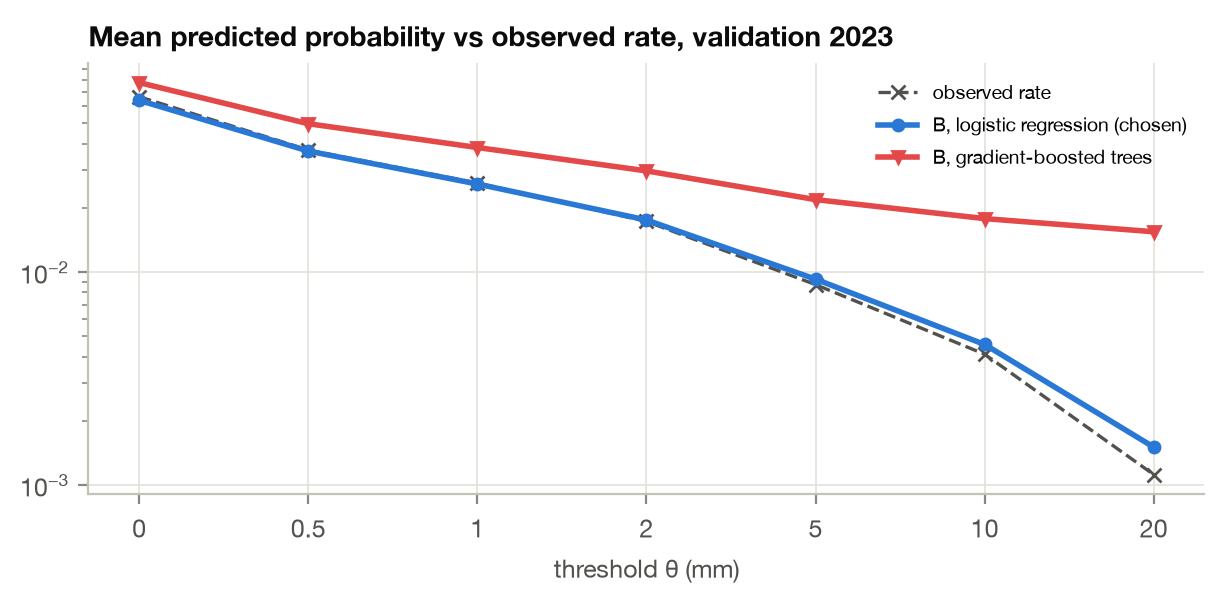
\includegraphics[width=0.7\textwidth]{fig15_gbt_calibration.png}
\caption{Validation 2023: mean predicted probability and observed event rate at each threshold $\theta$ (log scale),
for the chosen Model B (logistic regression) and its gradient-boosted alternative. The logistic regression follows the
observed rate; the trees over-predict, and more so at higher $\theta$. \src{src/plot\_task2.py from src/task2\_train.py}}\label{fig:gbt}
\end{figure}

\subsection{Task 2: the test year 2024 (evaluated once)}
We ran the test once, at \val{test_started}, with the plan unchanged since it was fixed and the chosen models loaded
from disk without refitting. Table~\ref{tab:testpooled} gives the pooled results and Table~\ref{tab:test} the results
per threshold.

\begin{table}[H]\centering\scriptsize
\begin{tabular}{lrrrrrrr}
\toprule
Model (test 2024, once) & AUC-ROC & AUC-PR & Brier & BSS & Log loss & Mean $p$ & $p$ rises with $\theta$ \\
\midrule
Climatology baseline & 0.798 & 0.085 & 0.02095 & 0.035 & 0.0950 & 0.0212 & 0.00\,\% \\
Persistence baseline & 0.865 & 0.404 & 0.01507 & 0.305 & 0.0674 & 0.0216 & 0.00\,\% \\
A: logistic regression & 0.806 & 0.084 & 0.02096 & 0.034 & 0.0925 & 0.0212 & 0.00\,\% \\
B: logistic regression & 0.959 & 0.654 & 0.01186 & 0.453 & 0.0478 & 0.0219 & 0.00\,\% \\
\bottomrule
\end{tabular}

\caption{Test year 2024, evaluated once: the chosen models and both baselines, weighted, pooled over $\theta$. \src{src/task2\_test.py}}\label{tab:testpooled}
\end{table}
\begin{table}[H]\centering\scriptsize
\begin{tabular}{lrrrrrrrrr}
\toprule
$\theta$ (mm) & Base rate & Clim.\ AUC-PR & BSS & Pers.\ AUC-PR & BSS & A AUC-PR & BSS & B AUC-PR & BSS \\
\midrule
all & 0.0222 & 0.085 & 0.035 & 0.404 & 0.305 & 0.084 & 0.034 & 0.654 & 0.453 \\
0 & 0.0635 & 0.119 & 0.024 & 0.522 & 0.362 & 0.115 & 0.022 & 0.740 & 0.500 \\
0.5 & 0.0362 & 0.072 & 0.016 & 0.464 & 0.317 & 0.071 & 0.015 & 0.705 & 0.493 \\
1 & 0.0256 & 0.052 & 0.011 & 0.407 & 0.263 & 0.052 & 0.011 & 0.640 & 0.435 \\
2 & 0.0169 & 0.036 & 0.007 & 0.331 & 0.194 & 0.036 & 0.008 & 0.547 & 0.343 \\
5 & 0.0084 & 0.019 & 0.003 & 0.229 & 0.110 & 0.020 & 0.005 & 0.427 & 0.236 \\
10 & 0.0038 & 0.010 & -0.000 & 0.151 & 0.057 & 0.010 & 0.002 & 0.330 & 0.150 \\
20 & 0.0010 & 0.003 & -0.002 & 0.063 & 0.012 & 0.004 & 0.000 & 0.192 & -0.008 \\
\bottomrule
\end{tabular}

\caption{Test 2024 per threshold: AUC-PR and Brier skill score (BSS) of the baselines and the chosen models. B's
AUC-PR stays far above the base rate at every threshold, but its BSS falls to about zero at the top one. \src{src/task2\_test.py}}\label{tab:test}
\end{table}

Model B's validation results held on the new year. On 2024 its AUC-PR is \val{t.B.all.aucpr} (validation
\val{v.B.all.aucpr}), against \val{t.pers.all.aucpr} for persistence and \val{t.clim.all.aucpr} for climatology. Its
Brier skill is \val{t.B.all.bss} (validation \val{v.B.all.bss}), against \val{t.pers.all.bss} for persistence and
\val{t.clim.all.bss} for climatology. Model A again sits at the level of climatology: AUC-PR \val{t.A.all.aucpr}
against \val{t.clim.all.aucpr}, Brier skill \val{t.A.all.bss} against \val{t.clim.all.bss}.

B's skill falls as the event gets rarer (Table~\ref{tab:test}, Figure~\ref{fig:thr}). Its AUC-PR is
\val{t.B.0.aucpr} for any rain, \val{t.B.5.aucpr} for more than \val{example_th}\,mm and \val{t.B.20.aucpr} for more
than \val{grid_max}\,mm, against base rates of \val{t.B.0.base}, \val{t.B.5.base} and \val{t.B.20.base}. At the top
threshold B still ranks the downpours far above the base rate and above persistence (AUC-PR \val{t.pers.20.aucpr}),
but its Brier skill is about zero (\val{t.B.20.bss}, against \val{t.pers.20.bss} for persistence): the probabilities
it gives are no more accurate than the base rate itself, and slightly less accurate than persistence. A downpour within half an hour is hard to
foresee from rain gauges alone.

Pooled over thresholds, B's probabilities are close to calibrated (Figure~\ref{fig:rel}). In no reliability bin does
the mean prediction differ from the observed frequency by more than \val{t_rel_B_maxgap}.

\begin{figure}[H]\centering
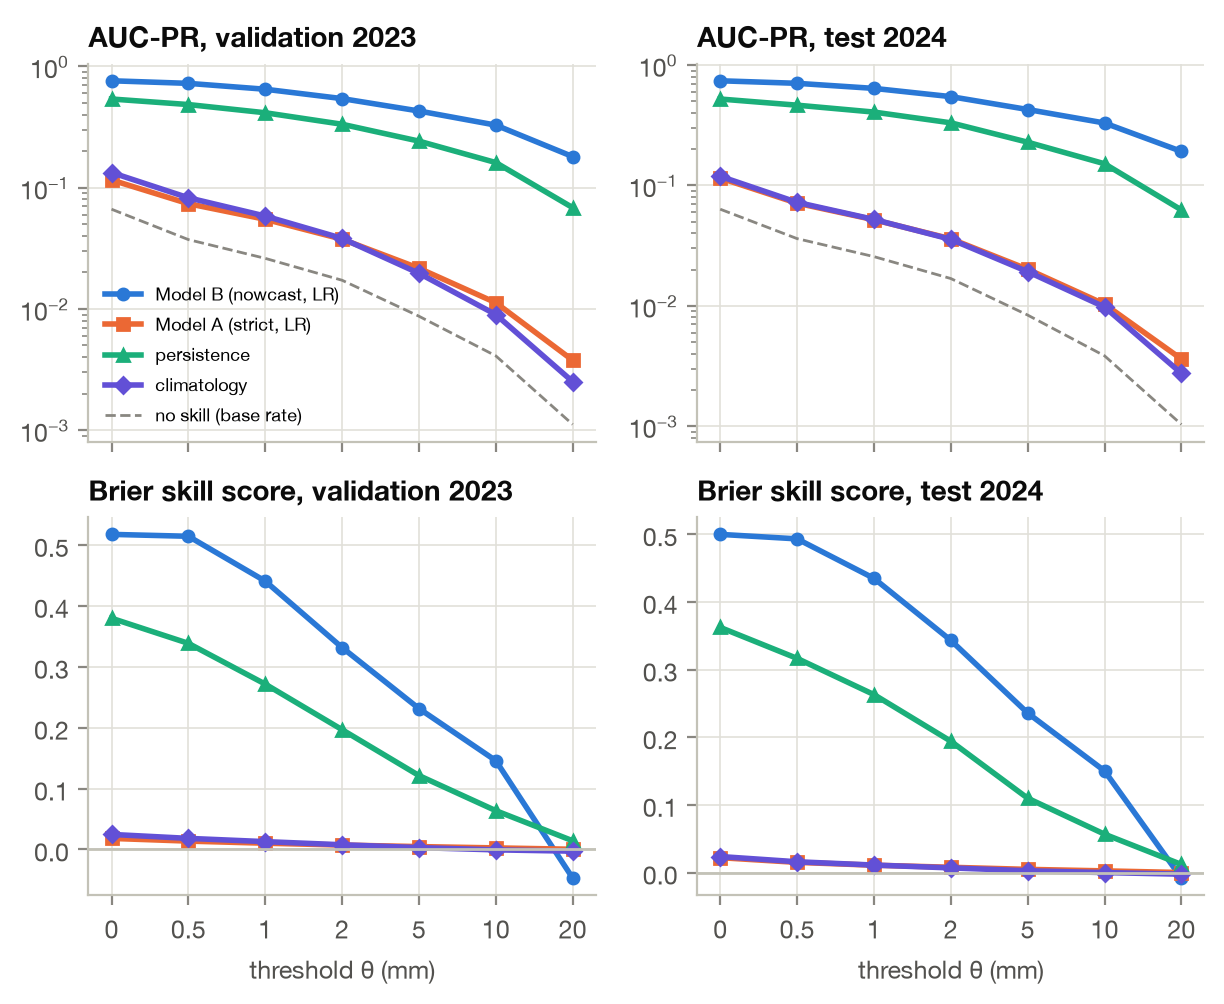
\includegraphics[width=0.8\textwidth]{fig12_per_threshold.png}
\caption{AUC-PR (top, log scale; dashed line: the base rate, i.e.\ no skill) and Brier skill score (bottom) at each
threshold, validation 2023 (left) and test 2024 (right). The two years look alike. B leads on AUC-PR at every
threshold, while its Brier skill drops to about zero at \val{grid_max}\,mm. \src{src/plot\_task2.py from src/task2\_train.py and src/task2\_test.py}}\label{fig:thr}
\end{figure}
\begin{figure}[H]\centering
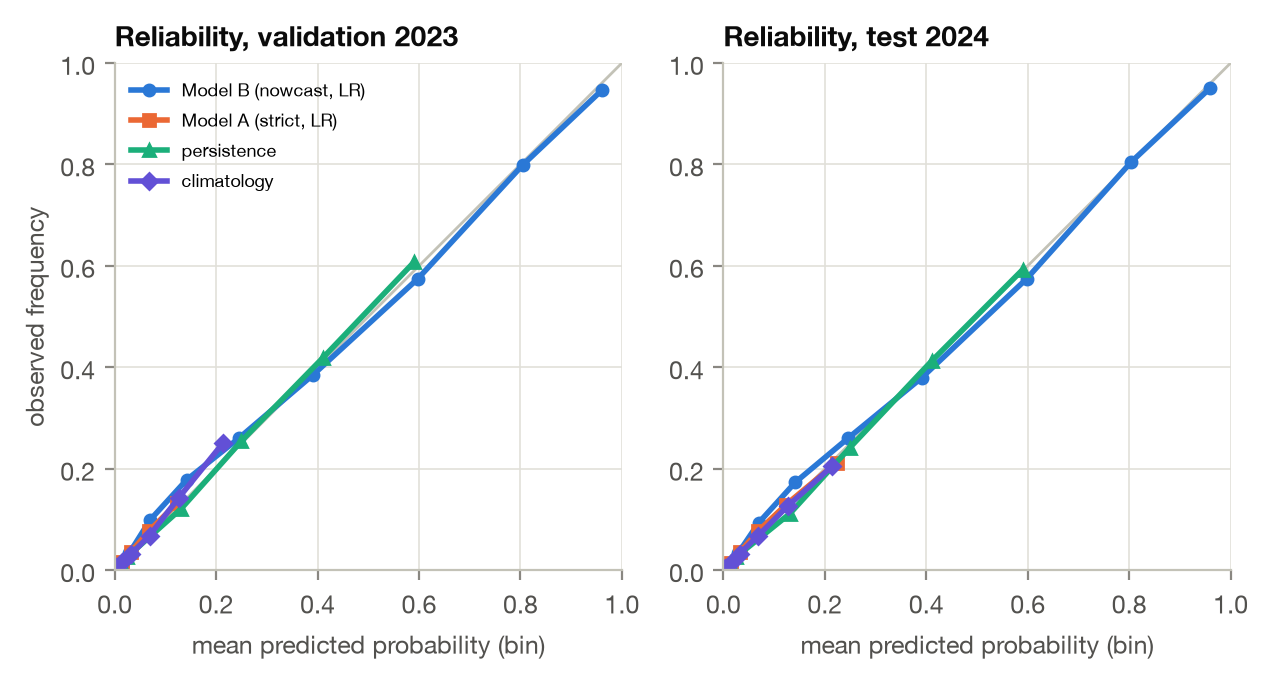
\includegraphics[width=0.72\textwidth]{fig13_reliability.png}
\caption{Reliability, validation 2023 (left) and test 2024 (right): observed frequency against mean predicted
probability per bin, pooled over thresholds (bins with at least \val{rel_min_rows} rows). A calibrated model lies on
the diagonal; B stays close to it up to the highest bin. \src{src/plot\_task2.py}}\label{fig:rel}
\end{figure}

Figure~\ref{fig:coef} shows what Model B relies on, as standardised coefficients: the change in log-odds for a
one-standard-deviation change in each input. Apart from the threshold terms, which set how the probability falls with
$\theta$, the largest are
\begin{itemize}
\item the time since the station was last wet (\val{coefB.mins_since_wet});
\item the island-wide maximum \val{horizon}-minute total (\val{coefB.isl_max_r30});
\item the island-wide share of stations that were wet in the last \val{horizon} minutes (\val{coefB.isl_wet30}), with
the share wet at $t$ close behind;
\item the station's rain in the last five minutes (\val{coefB.log1p_r5}).
\end{itemize}
Rain at the station and across the island up to $t$ is what makes the next half hour predictable. The hour and
day-of-year terms are much smaller once these are known.

\begin{figure}[H]\centering
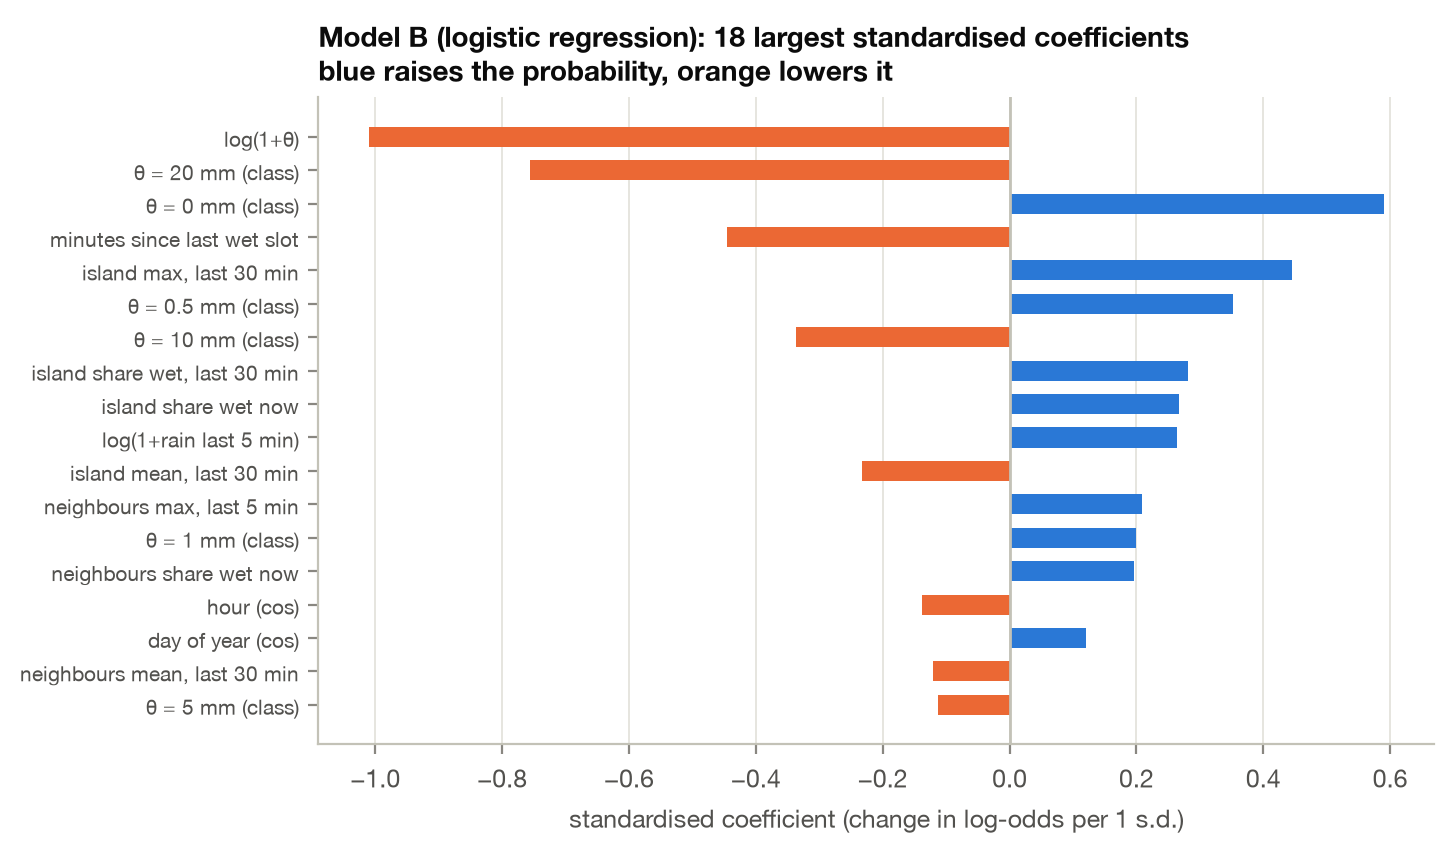
\includegraphics[width=0.72\textwidth]{fig14_coefficients_B.png}
\caption{Model B (logistic regression): the \val{n_coef_shown} largest standardised coefficients, as change in log-odds
per standard deviation of the input (blue raises the probability, orange lowers it). After the threshold terms, recent
rain at the station and across the island dominates; the calendar terms are small. \src{src/plot\_task2.py from src/task2\_coefficients.py}}\label{fig:coef}
\end{figure}

% ======================================================================================================
\section{Declaration of AI use}
\req{E11}
We used Claude Code (Anthropic, Claude Opus 5.5) as a coordinating session and a delegated builder session to plan the
work, write and run the Spark ingestion, cleaning, analysis and MLlib code, run the experiments, verify the data
against official records and draft this report. We directed the work and are responsible for the content and quality
of this submission.

% ======================================================================================================
\section{Additional work, observations and limitations}
\req{E12}
\subsection{Additional work}
\begin{itemize}
\item We checked the dataset against the official MSS daily station records (Section~\ref{sec:mss}). This is how we
found the January 2021 outage and the months in Table~\ref{tab:gapmonths}.
\item We recomputed the annual totals and the frequency and intensity indices on a fixed panel of \val{panel_n}
stations, to separate changes in rainfall from changes in the network (Figure~\ref{fig:annual}).
\item Before relying on each pipeline check, we fed it a deliberately broken input and confirmed that it stopped the
run (\code{checks/qualify.py}): a missing year, one unaccounted row in the cleaning ledger, a random split, an edited
analysis plan, a second test run, a 2024 row in the fitting table, and a hand-typed number in this report. The log is
\code{outputs/qualification/qualification.log}.
\item Before the single 2024 run, we ran the test script on 2023. It rebuilt the validation sample row for row, so we
knew the test path worked before it touched 2024.
\end{itemize}

\subsection{Limitations}
\begin{enumerate}
\item \emph{Gaps are not random.} A network outage on \val{jan21_gap_days} 2021 removed the wettest days of a record
month, and single stations fall silent for weeks at a time. Rates over reported slots cannot recover rain that was
never recorded, so the months in Table~\ref{tab:gapmonths} are misstated: most read too dry, and January 2023 too wet.
\item \emph{No quality control in the source.} Some complete days are simply wrong: a gauge reports zero through a
storm, or reports a day of rain that never fell (\val{mss_spur.st} on \val{mss_spur.date}). In all, \val{mss_big20}
station-days differ from MSS by more than \val{heavy_hour_mm}\,mm. Every value on such a day is plausible on its own,
so our rules cannot flag the day without an outside reference. These days remain in both tasks, but there are too few
of them to change the extreme-rain counts (Section~\ref{sec:mss}).
\item \emph{Measurement change in 2020.} The share of positive readings on the \val{gauge_step}\,mm grid drops from
\val{mult02.2019} in 2019 to \val{mult02.2021} in 2021. The fixed panel holds the stations constant, not the
instruments, so it cannot show whether this change moved the across-year results. Statistics of small amounts, such as
the share of very light rain, are the most likely to be affected.
\item \emph{Eight years.} The across-year differences (a dry 2019, wet years in 2020--2022) are in the data, but eight
years cannot separate a trend from natural variability such as ENSO and the Indian Ocean Dipole.
\item \emph{Model A is limited by its inputs, not by MLlib.} Under the strict reading of the brief, the station, the
time and the threshold carry little information about the next half hour, so Model A ends up as a calibrated
climatology.
\item \emph{Model B needs live data.} It uses the station's and its neighbours' readings up to $t$, so it only works
where those arrive in real time. If the station has no reading at $t$, \code{predict.py} falls back to Model A.
\item \emph{Sampling.} The models were fitted on a weighted sample of prediction times (Section~\ref{sec:t2model}),
not on all \val{f30_rows} labelled training times. The trees in particular might gain from more rows; we did not test
this.
\item \emph{Calibration of the trees.} A calibration step fitted on 2023 might remove the trees' over-prediction and
let them beat logistic regression on log loss as well. We did not try it: the plan fixed before fitting had no such
step, and adding one after seeing 2023 would have meant tuning on the validation year.
\item \emph{Cloud security.} The Dataproc nodes had public IP addresses, which the cluster needed to download the data from data.gov.sg itself, and Google warned that the project's default network firewall allowed ingress from any address. The clusters existed only for this run and were deleted afterwards, with a 30-minute idle limit as a backstop.

\end{enumerate}

% ======================================================================================================
\section{Submission contents}
\req{E13}\req{E14}
\begin{itemize}
\item \code{README.md}: setup, every stage in order with its runtime, how to load and use the trained models, the
Dataproc script and the checks.
\item \code{src/} (pipeline), \code{checks/} (the checks that stop the pipeline on bad input), \code{config/} (the
analysis plan fixed before fitting, and the record of the single test run), \code{cloud/} (Dataproc).
\item The trained models: \code{models/model\_A} and \code{models/model\_B}, saved with \code{PipelineModel.save}. Use
\code{src/predict.py -{}-station S24 -{}-time 2024-06-01T15:00 -{}-threshold 0.5 5}.
\item This report, built with Tectonic from \code{report/}, with every number generated into \code{report/generated/}.
\end{itemize}

\end{document}
